
% !Mode:: "TeX:UTF-8:Hard"
\ifx \allfiles \undefined
\documentclass[a4paper,12pt,twoside]{book}
%\usepackage{CJKutf8}
\usepackage[T1]{fontenc}
\usepackage{pifont}
\usepackage{graphicx}
\usepackage{capt-of}
\usepackage{color}
\newcommand{\linuxcommand}[1]{\texttt{\textcolor{blue}{\$ #1 \Pisymbol{psy}{191}}}}
\newcommand{\op}[1]{\textcolor{blue}{-#1}}
\newcommand{\hotkey}[1]{\framebox{#1}}
\newenvironment{screen}{\sffamily}{\rmfamily}

\usepackage{listings}
\definecolor{mygray}{rgb}{0.9,0.9,0.9}
\lstset{backgroundcolor=\color{mygray}, basicstyle=\small}
\lstset{morecomment=[s][\color{red}]{/*-}{*/}}
\newcommand{\Hilight}[1]{\makebox[0pt][l]{\color{yellow}\rule[-3pt]{#1em}{11pt}}}
\newcommand{\HilightLine}[2][yellow]{\makebox[0pt][l]{\color{#1}\rule[-4pt]{#2em}{13.9pt}}}


\begin{document}
%\begin{CJK*}{UTF8}{song}
\title{basic knowledge}
\author{yan zhao}
\date{}\maketitle

\tableofcontents

\else
\chapter{Developing Knowledge and Tool}
\fi

\section{Linux basic}
\begin{itemize}
		\item There is a good artical to introduce Linux distribution. \textbf{The name is "RedHat vs Debian : Administrative Point of View".} You can google and read. In one word. RedHat is stable, commercial server with small amount of packages. Fedora and CentOS are based on it. Fedora is cutting edge implementation(For test). Another big group is Debian, It's also stable with much more packages. Ubuntu is based on Debian.

		\item Ubuntu is for desktop, and Mint is sleek and quick version of Ubuntu, CentOS is for server, It's stable. \textbf{If you use virtual machine, recommend Mint, if you want to install linux directly on a computer, you can use Ubuntu system.}, because it's more friend toward beginner. 

\item There are two Interface Framework, Qt and GTK\@.  KDE is based on QT, and Gnome and Cinnamon(Mint) is based on GTK.  

\item You can use \linuxcommand{uname} to check basic information about your computer, detail can be seen uname --help. 

\item \linuxcommand{lscpu} will tell you how many cores do you have. Socket is physics CPU, "cores per socket" is number of cores. 
\end{itemize}

\subsection{Terminal tips}

 \begin{itemize}
  \item Move shortcut keys are list below:Ctrl+p or up down arrow key can go to the previous command, this is very useful. 
\begin{center}
  \begin{tabular}{c|c}
 \hline shortcut & function \\
\hline Ctrl+f,b & forward, backward character \\
\hline alt+f,b & forward, backward word \\
\hline Ctrl+a,e & move start,end \\
\hline Ctrl+p,n & previous, next line \\
\hline Ctrl+r & search command history \\
 \hline
  \end{tabular}
\end{center}

\item delete shortcut keys: You can use "hw" to delete previous character or word. "dd" use to delete forward character or word, "uk" to sentence begining and end. In Vim, the keyboard shortcut is not the same. 
\begin{center}
  \begin{tabular}{|c|c|}
 \hline shortcut & fucntion \\
 \hline \textbf{Ctrl+l} & clear the screen \\	
\hline ctrl+k,u & delete to begin/end \\
\hline alt+d,backspace & delete forward/backward word \\
\hline Ctrl+d,h  & delete forward/backward a character  \\
 \hline
  \end{tabular}
\end{center}

\item You can remember "eu" "ak". They both delete the whole line, The first letter is move command. And the second letter is edit commmand. 

\item bind -p will list all the shortcut

\item  About keyboard shortcut, I have good idea, that is to use left Ctrl and Alt together, because you can use your thumb to press Alt and use palm to
	press Ctrl\_L,(Even in my three laptops, I also can press Ctrl\_L easily by palm).
	So a shortcut can be defined below:
	\[ \left\{ \begin{array}{cl}
	            \textrm{move} & \left\{ \begin{array}{c} \textrm{other: Ctrl\_L} \\ \textrm{emacs: Alt\_L} \end{array}  \right. \\
		    \textrm{select} & \left\{ \begin{array}{c} \textrm{other: Ctrl\_L+Shift\_L} \\ \textrm{emacs: Alt\_L+Shift\_L} \end{array}  \right. \\
	           \end{array} \right. + \left\{ \begin{array}{c}
						\textrm{left character: J} \\
						\textrm{right character: L}\\
						\textrm{upward: I}\\
						\textrm{downward: k}\\
						\textrm{left word: U}\\
						\textrm{right word: O} \\
						\textrm{begin line: H}\\
						\textrm{end line: ;}\\
						\end{array} \right.
	\]
	Delete command is below: \\
	\[ \textrm{delete} \left\{ \begin{array}{l}
	            \textrm{left character: Backspace}  \\
		    \textrm{right charcter: Ctrl\_L+N} \\
		     \textrm{left word: Ctrl\_L+Backspace}  \\
		    \textrm{right word: Ctrl\_L+M} \\
		     \textrm{line: Ctrl\_L+P}  \\
	           \end{array} \right.
	\]
	

	Question 1: why always left Ctrl?  \\
	Answer: Now, if you are smart enough, you can found that there is rules inside. All the commands is left Ctrl add right hand character, becuase left Ctrl can be
	pressed by left palm and right hand is more flexible than left hand when you click the different character. \\

	Question 2: why other use Ctrl and Emacs use Alt. \\
	Answer: In common applications, Alt has been assign to trigger menu item, such as Alt+F will trigger File menu, so, I must use Ctrl. In Emacs, on the contrary,
	Ctrl has been used to trigger some common commands, so I use Alt key( and Alt is used not often as Ctrl).\\

	Question 3: How can I export my custom shortcut to other computers \\
	Answer: There are two kind of shortcut one is kate and other is kile, they store in \verb=.kde/share/apps/katepart/katepartui.rc= and \linebreak[4] \verb=.kde/share/apps/kile/kileui.rc=
	you can copy them and cover them in your computer. If version is different, Maybe it's a little difficult. But you can just do it within the application, it don't need very long time. \\
        \\
	By now, these customized shortcuts haven't been used in practical use. Anyway, you can use arrowkey, it don't need too much memory. But it is a good suggestion. You can learn how to define a customized shortcut. If you need to do a lot texting job, they are very useful.
	 %目前,这些键盘的定义我还没有在实践中使用过。毕竟,用箭头键太直接了,而按住ctrl在一些笔记本上不是太方便。 不过,他们依旧是一个很好的建议,以后当你使用大键盘,或者是比较密集的进行编辑工作的时候,还是非常值得尝试一下的。
  \item Ctrl+Alt+F1\ldots F6 switch terminal. Ctrl+Alt+F7 return back to GUI\@. When F7 doesn't work, you can try F8. 
\end{itemize}

\subsection{time}
\begin{itemize}
\item For linux file time: there are three time stamps: atime (access time), it is when the file was last read.\  ctime is the inode change time, while mtime is the file modification time.\  mtime changes when you write to the file. It is the age of the data in the file. \textbf{Whenever mtime changes, so does ctime, except you use touch command} But ctime changes a few extra times. For example, it will change if you change the owner or the permissions on the file.  

\item  timestamp will be used in many linux commands, ls -l will show modification time. and you can use \linuxcommand{stat fileName} to see all the three time. The can be used in find command. 

\item \linuxcommand{touch} can change time of a file or you can use it to produce an empty file.  \linuxcommand{touch -a existFile} change access time and ctime. \linuxcommand{touch -t existFile} change modify time and ctime.   \linuxcommand{touch -c existFile} change a,c and m time. 
            
\item \linuxcommand{touch -t YYMMDDHHmm} will set mtime and atime to the date you want and it sets ctime to \textbf{NOW}. You have complete control over mtime, but the system stays in control of ctime. So mtime is a little bit like the date on a letter while ctime is like the postmark on the envelope. System use ctime to do backup job. An example can be found in my evernote book mark. 

\end{itemize}


\section{File and Dir}
\subsection{basic}
\begin{itemize}
\item A hard link points to the file by \textbf{inode}.  A symbolic link points to the file by \textbf{filename}. 
 
\item  There is no "real" hard link name; All hard links are equally valid names for the file. You can use \linuxcommand{ls -l}. The first number after the file mode is the link count(this count is represent hard link number).  For symbolic link, It just point to a filename, If origin file name changed, symbolic link will not be valid.   symbolic is very flexible,  It can be linked to a dir or it can be linked to different file system. but hard link has many restriction. 

\item \linuxcommand{find -L / -samefile path/to/foo.txt}find all files links to foo.txt

\item Absolute directory must begin with root directory /
		

     \item Linux don't use extension name to specify file type, you should use \linuxcommand{file fileName} to judge it. 
     
	 \item When you use ls -l, the first character stands for different kinds: -:file, d:Dir,
         l:link file, b:interface of device. So you can use \linuxcommand{ls -al | grep \^{}d} to show all the directories. 
	 
    \item \linuxcommand{ls -d */} will list only directory without all files in it. if you want to see all files in it. omit -d
 
   \item /usr stands for UNIX Software Resource, isn't user. It associate with software. /users includes all the users name, don't confuse them. installing and executing. FHS recommend linux developer install their application into the different dirs inside of /usr:  such as /usr/bin and /usr/lib. Don't build their separately directory.  For example, when you install codeblock, you can see codeblock exe file in /usr/bin. when you \linuxcommand{ldd codeblock}. you can see it use a lot of lib in /usr/lib. There is no codeblock directory which includes everything.  It's different with Window system.
         \item /var include all cache, log, mail which are increased when you system is running. so it will increase with time. 
         
     \item The Dir Structure:\\
\begin{tabular}{p{0.2\textwidth}|p{0.7\textwidth}}
  \hline
  % after \\: \hline or \cline{col1-col2} \cline{col3-col4} ...
  /bin & includes important comands: mv, mkdir, chmod, cat, chown and date  \\
 \hline  /etc & Main configuration file: /etc/init.d/ /etc/fstab \\
  \hline /home & home directory \\
  \hline /opt & just like /usr/local  \\
  \hline /usr & /usr/local install some your own software, /usr install OS software.  /usr/bin, /usr/include(c++ language), /usr/lib(c++ language),  /usr/src \\
  \hline /tmp & any body can access or write it.     \\
  \hline /srv & web service(www and ftp) access data \\
  \hline /sbin & root command \\
  \hline /proc and /sys & virtual file system, they are stored in memory.  proc and kernerl information \\
  \hline /dev & device file \\
  \hline /lib & lib used when you start linux. /lib/modules has kernel modules \\
  \hline 
\end{tabular}

\end{itemize} 
\subsection{partition and mount point}
	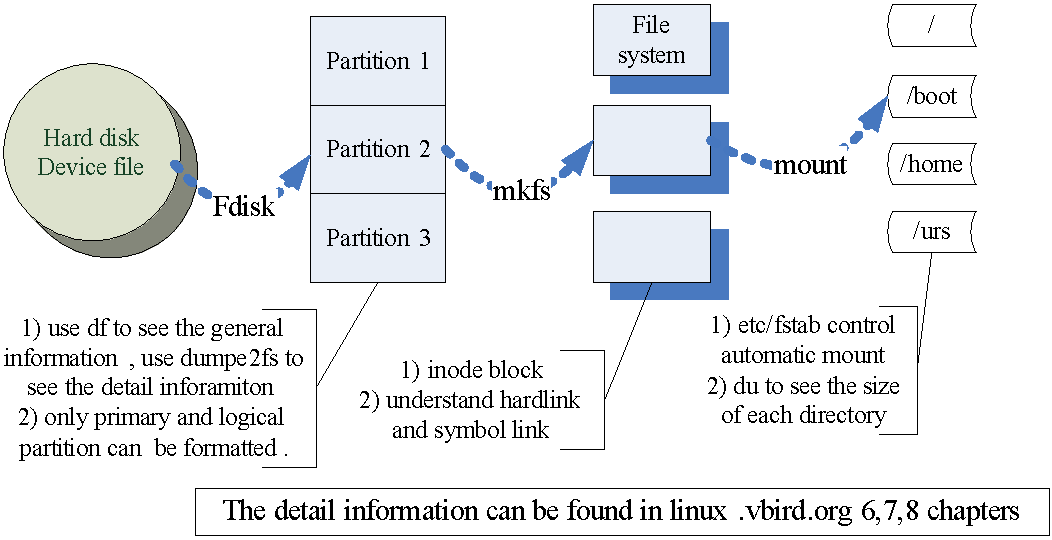
\includegraphics[scale=0.8]{pics/basic_file_system_clip}
	\\ 
   A good tool software in linux system is GParted, which  is used for creating, deleting, resizing, moving, checking, and copying disk partitions and their file systems.  You also can use df command to check your system \textbf{partitions}. You can create 1) partitions by GParted 2) mkdir a dir 3) then mount them by adding below text in /etc/fstab file.    \\   
   \verb=/dev/sda3 /home/yan/llvm ext4 defaults 0 0=
   
   \textbf{/etc, /bin, /dev, /lib and /sbin can NOT be put in different partition with root /. }  \\

\subsection{permission or file mode}
\begin{itemize}
      \item \linuxcommand{ls -al} will list all the files ownership and permission. Basiclly, all the system support \linuxcommand{ll} command directly. 
			  
  \item There are three different groups: owner, Group, and Other. In each group,  there are three different permissions: r, w, x;

  \item for File and Dir, "rwx" has different meaning. x for Dir means you can come into this dir.  For a Dir, if you only have r permission, you only can \linuxcommand{ls -l Dir}, You can't cp a file from it unless you have x permission. So x permission is very important for a Dir
		  	
      \item \linuxcommand{chown chgrp} are very useful when you copy files to other peoples. \linuxcommand{chgrp -R grpName dirName}, you must make sure grpName in /etc/group file. or it will report error.  \linuxcommand{chown} command need to make sure owner name in /etc/passwd file. 

          \item When you need to use chgrp or chown? When you copy a file to other people. 

		  \item \linuxcommand{chmod} command follow[ugoa][+-=][rwx], for example, \linuxcommand{chmod u+x file}  or \linuxcommand{chmod go=r file}. there are four letters: u(owner), g(group), o(other) and a(all).\textbf{u represent owner, You need to remember that specially}. ("=") means "set the permissions exactly like this.
		  \item SUID or GUID, In simple words users will get file owner’s permissions as well as owner UID and GID when executing a file/program/command. An good example is passwd command, It's owned by root, When you launch it, you have root permission to modify /etc/shade file. That is all!
\end{itemize}


\subsection{commands about File}
\begin{itemize}
		\item \linuxcommand{du -h} command displays the sizes in kilobytes of all files in the specified directory.  df command displays the amount of unused space left in your disk system. \linuxcommand{du -sh *} will show your every directory size. \linuxcommand{du -sh * | sort -h} will sort all directory size. Don't use sort -n here, it will put 1.1G ahead 1.2M. 

\item \linuxcommand{pwd} return where you are

\item \linuxcommand{cd -} will return the previous path

\item \linuxcommand{diff a.cpp b.cpp} will show line-by-line differences. 

\item In GUI, you can drag a file into terminal. 

\item when you run a command, sometimes you need to \linuxcommand{./a.out}. "./" means current directory.
		
    \item When you use cp, you need pay attention to -a options, it related to maintains permission and owners.

        \item You can use \linuxcommand{od} to see the binary file, It reminds me the UltraEdit
        
        \item \linuxcommand{rmdir} only can be used to delete an empty dir. You can use rm -r to delete a directory with files in it.

            \item \linuxcommand{tail, head, cat ,tac, less } less will stop, to ask you to continue. Maybe less is better than cat.  I often copy-and-paste text from the web into a file like this (command prompt shown):
                \begin{verbatim}
                $ cat > filename
                <Cmd-V>
                <Ctrl-D>
                \end{verbatim}
            \item \linuxcommand{which -a command} will help you find command's name and in all \$PATH directory.  \linuxcommand{type} can tell you if a command is bash build in command. such as cd command.  They are used to know more about your commands

             \item \linuxcommand{file} is to determined the kind of all files.( executable, text, or data file).  
                
             \item \linuxcommand{locate} can help you find a file very quickly, because it just search in an index database.   you can use \linuxcommand{updatedb} to update this database. \linuxcommand{whereis} just look for binary(-b option) or source(-s option) files. They just used to search binary and source files. 

                 \linuxcommand{find} to perform a throughout search, usage is complex, see below.   
                 
\end{itemize}

\subsection{find command}
\begin{itemize}

	  \item \linuxcommand{find . -name "tex*"} can help you find all tex* file from current directory recursively. It's a very powerful command, without -name, it will search all the files.  Don't forget double quote around tex*. It will give tex* directly to find command. if you don't do that, shell will expand it by itself. and it will not search recursively. 
	  \item \linuxcommand{find .-iname "Abc*"} will ignore letter case. 

	  \item You can find according to \textbf{name, type ,size, owner and time. } You also can use logic or operator.
	  	  
     \begin{enumerate}
     	  \item \linuxcommand{find ./dir -maxdepth 1 -type d -iname "man*" } -type can be b(block), c(characer special file) d(directory), p(pipe), l(symbolic link) s(socket), or f(plain file).  

     	  \item \linuxcommand{find ./dir !(-not) -iname "man" } use ! or(-not).  ! or(-not) means to exclude "man" 

     	  \item \linuxcommand{find ./dir -name '*.php' -o -size +20M} Default it AND, if you want to use OR, use -o.  

     	  \item \linuxcommand{find \$HOME -ctime -2 -name "*.cpp"} -ctime(-cmin) +n|-n|n: Find files that were changed more than n (+n), less than n (-n), or exactly n days ago. cmin is minutes. About ctime and mtime, can be seen previous explanation. 

     	  \item \linuxcommand{find . -size -50M -size +20M}  c:bytes, k:kbyte, M:Mbyte G: b:512-byte blocks. Find all files smaller than 50M and bigger than 20M. 

     	  \item \linuxcommand{find . -user yan -group UH -perm 644}, see -user, -group and -perm. 
     	  
		  \item for symbolic link, you can see -H, -P, -L options in find command man page. default is -P, means that Never follow symbolic links.

\item \linuxcommand{find . *.txt} and \linuxcommand{find . "*.txt"} are different. In the first example, shell will receive *.a and expand it to a.txt b.txt c.txt.... In the second example, find command receive *.a.  So the first find command, If in your current directory, there is a.txt. find will not look all *.txt recursively.  

\item \linuxcommand{find . "ab"} will not find "abc" file. You need to use "ab*" to get it. A better expression is "*ab*" will find more files. 


\item In the previous example, you also can use \linuxcommand{find . $\backslash$*.txt}. Use $\backslash$ to escape the original means. 

\item Sometimes, find will output "Permisson denied". You can use below command to filter these message. 
\begin{verbatim}
in bash:
find / -name art  2>&1 | grep -v "Permission denied"
in csh:
find / -name art |& grep
\end{verbatim}

  \end{enumerate}
  
  \end{itemize}
\subsection{grep command}
\begin{itemize}
		\item \linuxcommand{grep -r -w -i "match" file1 file2}.\textbf{Put files name in the end. That is basic pattern. If it's a directory, add -r after grep. }

		\item You can give a directory name. But you must add -r option if you input a directory name. \linuxcommand{grep -r 'word' .} 

		\item -n will give match line number. Once you know line number, you can vim +num file to open it.  
		\item -v inverse result. -l will supress your output. It will only output file name. -l will help you to deal with file with some pipe command, such as copy or rm files with some match words in them.  
	
		\item A, B, C use to print line aroud match. \linuxcommand{grep -B 2 -A 1 'computer' file}
				

\item \linuxcommand{grep --include=$\backslash$*.\{c,h\} -rnw  -e "pattern" /path} -w stands match the whole word. -l (letter L) can be added to have just the file name. This will only search through the files which have .c or .h extensions. Similarly a sample use of --exclude: 

\item \linuxcommand{echo i*} or \linuxcommand{ls i*}, first, shell will look for all filename which begin with letter i,\textbf{It will not replace * with all file names and add i in front of it}. If it fail, it will print out "No match"

\item \linuxcommand{echo --include=*}, just like previous example, it will fail to look for filename begin with --incl.. So it will print out No match. If you use \linuxcommand{echo --include=$\backslash$*}, it will print literal string out.

\item \linuxcommand{echo --inclue=$\backslash$*.\{a,b\}} will output --include=*.a and --include=*.b
	 	
\item From all previous examples, if you use \verb!--include="*.{c,h}"!. It will prevent shell to expand * and big bracket. It's not right. For new version grep, You don't need double quote. --include will prevent shell expand. But for old grep, it doesn't work. I recommend to use \verb!--include=\*.{h,c}! to escape * symbol. It work on both new and old version.  

\item -c will only print  match number, -C3 will print context 3 line information .  

\item Since you usually type regular expressions within shell commands, it is good practice to enclose the regular expression in single quotes (') to stop the shell from expanding it. 

\item grep support regex, You need to use -E option to support extended regex. \linuxcommand{grep -E 'abc\{1,2\}d' file}.  that's very power feature. Here, I just list a few basic usage. 

\item \linuxcommand{grep 'word' *.txt} will just look for txt file in current directory. \linuxcommand{grep -r --include=\*.txt 'word' .} will look for all .txt file recursively. 

\item -e and -E follow regular expression. -e is basic version. In basic regular expressions the meta-characters \verb=?, +, {, |, (,)= lose their special meaning; instead use the backslashed versions \verb=\?, \+, \{,  \|, \(, and \)=. \textbf{I recommend to use -E option.}

\item basic regex syntax:

 \begin{tabular}{p{0.25\textwidth}|p{0.3\textwidth}|p{0.35\textwidth}}
\hline 
sytax 	& example & 	description \\

\hline 
\^{} (Caret)	& '\^{}smug'  & 	'smug' at the start of a line \\
\hline 
\$ &  'smug\$' & 	match expression at the end of a line\\
\hline 
$\backslash$ (Back Slash)&   '123$\backslash$\$'  Just looke for '123\$' in file. &	turn off the special meaning of the next character, as in \^{} and \$ \{.   \\
\hline 
[ ] (Brackets)	&'[0-9][0-9]' pairs of numeric digits &	match any one of the enclosed characters,  Use Hyphen "-" for a range, as in [0-9].  [\^{} ] means excludes\\
\hline 
. (Period) & '\^{}.\$' lines with exactly one character  &	match a single character of any value, except end of line. \\
\hline 
* (Asterisk), ? , + &  &	match zero or more*,  + (pluse) is one or more,   ?(question mark) is zero or one occurrence.   \\
\hline 
\{x,y\}, 	\{x\}	\{x,\} & &	\{x,y\}match x to y occurrences of the preceding;  or \{x\} x occurrence; or  \{x,\} x or more occurrences. \\
\hline 

\end{tabular}

\item When you mean match number, \verb=* equal ? and + = 

\item '[abc]+',  '(abc)+' and 'abc+' are different.  (abc) means it's a group, and should be considered as whole. abc+ means that + just used on letter c, So it will match ab or abc.  

\item '<.+>' will math "<car>...</car>". Default it use greedy match. If you want to use lazy match, use '<.+?>'. When you use '<.+?>'.  You should use \linuxcommand{grep -P '<.+?>'} -P means that use perl language standard. 

\item Usally, grep just match one line. If you want match multilines. You can use \linuxcommand{grep -Pnzo 'BLOCK($\backslash$n|.)*?END\_BLOCK }.  Pay attention it use lazy match method. and . doesn't means newline, you need to use '($\backslash$n|.)*?'

\item Differences grep and find:
		\begin{enumerate}
				\item grep put file names or directory name in the end, find just use directory after the find command.
				\item find don't need -r, it need recrusive automaticlly, grep must use -r if you follow a dir
				\item grep will partial match, find will not partial match unless you use *.
				\item \linuxcommand{grep -r --inlucde=$\backslash$*.\{a,b\} -E 'abc*' .} The first * is shell to expand file name, The second * is regular expression, stand for match zero or more. 
				\item find command pattern: \textbf{find dirname expre1 [or] expre2}, expre1 is -name '*.txt' expre2 is -ctime -2 
				\item grep pattern: \textbf{grep -rnw 'abc' *.txt}
		\end{enumerate}
\end{itemize}



\section{User}
\begin{itemize}
\item \linuxcommand{cat /ect/passwd} will tell you all the users and which shell they are using.
 \item Don't log in root, you can use \linuxcommand{sudo } follow your command
\item \linuxcommand{whoami} tell you account informaiton.
\end{itemize}



	


\section{shell}
\subsection{wild character and quote}
\begin{itemize}
\item Single quotes preserves the literal value of each character.  Double quotes preserves the literal value of all characters within the quotes, with the exception of '\$', 'backtick', '$\backslash$', and, when history expansion is enabled, '!'. 
\begin{verbatim}
echo '$PATH `pwd` '
echo "$PATH `pwd` \$PATH"
\end{verbatim}
\end{itemize}

\subsection{Environment variable}
\begin{itemize}
			
\item When bash is invoked as an interactive login shell, or as a non-interactive shell with the --login option, it first reads and executes commands from the file /etc/profile, if that file exists. Then/etc/profile.d/*.sh. Then it looks for ~/.bash\_profile,  ~/.bash\_login, and ~/.profile, in that order, and reads and executes commands from the first one that exists and is readable. The --noprofile option may be used when the shell is started to inhibit this behavior.
		

\item When an interactive shell that is not a login shell is started, bash reads and executes commands from  /etc/bash.bashrc and ~/.bashrc, if these files exist. This may be inhibited by using the --norc option. The --rcfile file option will force bash to read and execute commands from file instead of /etc/bash.bashrc and  ~/.bashrc.	

\item echo \$0 will show "bash", it's not login shell. if it shows "-bash", it is login shell.  
	
	\item Why we need variable, just like macro in C language. With varaible, we can config and customize an application outside. And we can customize a varaible to affect a lot of applications. such as \$PATH
				
	\item set: \linuxcommand{YanVar=123} unset: \linuxcommand{unset YanVar} check: \linuxcommand{echo \$YanVar}

	\item There are two kinds of variables: environment and user defined.

	\item \linuxcommand{env} shows all the environment variable. such as \$HOME,  \$PATH, \$LANG,\$EDITOR which can specify you default editor in your system.

	\item \linuxcommand{set} list all the local environment variables and user defined varaible , that is more than env command. For example, the \$PS1.  \linuxcommand{unset} to delete an environment variable

	\item \linuxcommand{getconf} can get some system variable, such as \linuxcommand{getconf ARG\_MAX}, you can use xargs -n 50 to make command satisfy the ARG\_MAX
	
	\item In mint, maybe in your home directory, there is no .bashrc file, so you need to create one and add export PATH=\$PATH:/home/yan/openuh-install/bin  then exit the current terminal and restart a new one. Then use echo \$PATH to see if the directory has been added.
	
	\item In previous command, Linux use : but windows use ; why windows use different?

	
	\item \linuxcommand{export DEPART=Sale} and \linuxcommand{DEPART=Sale ; export DEPART} they means the same. If the export statement in a script file,
	you must use \linuxcommand{Source a.sh} or \linuxcommand{. a.sh} to run the script file, then It will affect the continuous processing. source means that this command only run in current bash, it doesn't run in a child shell.
	
	\item Every time when you open a new terminal, It will read .bashrc or .rshrcIt depends on what shell you are using, that is why you need to use \linuxcommand{echo \$0} to know which shell you are using. It will use export(bash) or setenv(csh) to load all envoriment variable. 
			

	\item If you alread in termial, you can use export or setenv command to add envoriment varaible. if these commands are in a sh file, you have to use \linuxcommand{source a.sh} to run. because, if no source command, it will open a child terminal, so after a.sh finish, child terminal will disappear, and all the environment varaible you just set in the child terminal will disappear too. 

	\item \linuxcommand{setenv} is csh command. In bash, you can use \linuxcommand{export} directly. \textbf{csh doesn't use =, bashrc doesn't use backslash.}
\begin{verbatim}
in .cshrc
setenv PATH $PATH\:/users/yzhao4/python-3.23/bin

in .bashrc
export PATH=$PATH:/storage/yzhao/binexport 
\end{verbatim}

\end{itemize}
	
\subsection{pipe}
\begin{itemize}
  \item pipe command can be called "filter", It will accept input fomr STDIN, perform operations, then send it to STDOUT. Such as grep, uniq, sort, fmt, pr, head, cut, tee, tr, join, paste, expand, split, tr, awk, sed, less

  \item You cann't judge if a command is filter by running it. cat will hang up to wait for you from STDIN, but less will show error message.

  \item xargs is also a filter, you can use this way \linuxcommand{find . -name "*.c" | xargs rm -rf } a.c and b.c will be rm command arguments.

  \item Sometimes, a command need a file name as input or output, but you don't want to give a filename, It usually used in pipe commands, such as \linuxcommand{gzip -dc a.tar.gz  | tar -xvf  - }. It just like \linuxcommand{gzip -dc a.tar.gz  | tar -xvf  /dev/stdin}

  \item "-" has nothing with shell, It's only available in tar command. Most of time, It's only used in tar. 
		  
\end{itemize}

\subsection{shell script}
\subsubsection{Basic}
\begin{itemize}
\item The first line of script is \verb=#!/bin/bash=.  This is a special clue given to the shell indicating what program is used to interpret the script. Other scripting languages such as perl, awk, tcl, Tk, and python can also use this mechanism.

\item After you finished script file, use \linuxcommand{chmod +x your-script-name}

\item echo -e "aaa$\backslash$nbbb" will output two lines

\item \linuxcommand{!!} run the previous command, \linuxcommand{!\$} is the previous argument. \linuxcommand{\$?} is the last bash command result, If it's 0, means that everything is OK. Detail can be found in google "Become a Command Line Ninja With These Time-Saving Shortcuts''

\item \linuxcommand{command1;command2}.   To run two command with one command line.  \linuxcommand{command1 \&\& command2} command2 is executed if, and only if, command1 returns an exit status of zero. \linuxcommand{command1 || command2} command2 is executed if and only if command1 returns a non-zero exit status.
\end{itemize}

\subsubsection{Variable} 

\begin{itemize}
\item \$0 is script name, and \$1, \$2.. are arguments to the scripts. 

\item print the contains of variable (HOME) and not the HOME. You must use \$ followed by variable name to print variables cotaines. \verb= echo $HOME= print the variable contents. and \verb=echo HOME= just print "HOME" string. It's a little confused for a C programmer, but you need to be used to it. 

 \item In most cases, \$var and \$\{var\} are the same: 

\item The braces are only needed to resolve ambiguity in expressions: such as echo \$\{var\}bar

\item \$(command) is same as `command. 

\end{itemize}

\section{processes}
\begin{itemize}
		\item CTRL-C aborts the app, CTRL-Z \textbf{suspend} app and put it to backgroud, you can use bg command to re-continue this job on backgound. CTRL-D is EOF. \textbf{C is cancel, D is end.}

 \item \linuxcommand{ps -l} and \linuxcommand{ps aux} are two common processes check command. ps aux will product a lot content, so we often use \linuxcommand{ps aux | grep user}. In status column, S is sleep, T is stop, and R is run. + symbol means it's in foregound. 

 \item \linuxcommand{./hello \&} will put hello to background. another useful commands are \linuxcommand{fg bg, job}. \textbf{They just belongs to this bash}. You can use ONE bash shell to do multi tasks. They are very helpful when you are login sever with ssh command. At this time, you only have one terminal window. So multi-task is import for you. If you work on local workstation. You can open another terminal windows easily, These commands are not very helpful for you.
 
 \item View all the background jobs using jobs command,  If you have multiple background ground jobs, and would want to bring a certain job to the foreground,  \linuxcommand{fg \%2} will bring the job\#2 and \linuxcommand{kill \%2} will kill it.  
 
 \item Ctrl-Z will suspend process. If you want to continue, you need to 1) use jobs to know its number, 2) use bg \%num to restart it in background. 3)3)3)If you want to bring it back to foreground, use fg \%num. 

 \item \linuxcommand{nice commandname \&} means that you run command friendly with other(not occupy all resources) and run it at background. Skuld may be a UNIX server!
	
 \item \linuxcommand{htop} will show processes dynamicly.

 \item \linuxcommand{kill -s singal PIDnumber} will send signal to processes with PIDnumber. \textbf{This command has some confusion with its name.}

 \item \linuxcommand{kill -l } will list all avaible singal, The default signal is TERM which allows the program being killed to catch it and do some cleanup before exiting. A program can ignore it, Specifying -9 or KILL as the signal does not allow the program to catch it, do any cleanup or ignore it.\textbf{It should only be used as a last resort.}
 
 \item \linuxcommand{ps -f --forest} will show all the processes in hierarchy.  Just like pstree

		 	
 \item I launch a background process, either by appending "\&" to the command line or by stopping it with CTRL-Z and resuming it in background with "bg". Then I log out.  We were quite sure it should have been killed by a SIGHUP, but this didn't happen; upon logging in again, the process was happily running and pstree showed it was "adopted" by init. But then, if it is, what's the nohup command's purpose? Below is answer: For BASH, this depends on the huponexit shell option, which can be viewed and/or set using the built-in shopt command.
\end{itemize}


\section{Application}
\subsection{Internet}
	\begin{itemize}
	\item You can google "where is my IP address'' to get you external IP, or use \linuxcommand{ipconfig} to know your internal IP. \linuxcommand{host} can know IP or host name from each other. Another Interesting tool is \linuxcommand{netstat} can tell you what connections are there in your computer. and \linuxcommand{traceroute} can trace the path in connection. They are some useful Internet connection tool.
	\end{itemize}
	

\subsection{VNC server}
\begin{itemize}
 \item It can help you to get remote linux desktop, It's very helpful for a windows programmer to use GUI in the linux host.
 \item vncserver -help will list all the command optoins.
 \item  You need to install VNC server in the linux with su priviliage, then run vncserver on the linux machine. Last on you windows machine, you can use putty and vncviewer to access the remote desk top. Detail can be googled, there are some reference pages available.
\end{itemize}


\subsection{clipboard}
	\begin{itemize}
			\item There are two kinds of clips: 1) normal clip, Ctrl+C copy and Ctrl+V paste. 2)Xclip, shift+mouse left button select+copy. Mouse middle button to paste. Most linux system support both. But they are two different clipboards. If you use Ctrl+C command, You can't use mouse middle button to paste it.
			
			\item \linuxcommand{xclip -o} will output content in xclip. Not normal clip.
					
			\item You just try xclip in shell to see if it's installed. if it's not installed, you can use \linuxcommand{sudo apt-get install xclip}. If you use Mac, in VMware fusion, you need to configure the Linux mouse setting.  default is command+primaryButton to simulate middle button.  xclip is very useful in linux, it support copy from a vim and paste to another vim.  
			\item How to use copy and paste in vim? you can see vim section for detail.
	\end{itemize}

\subsection{Installing}
	\begin{itemize}
	\item There are two kinds of installing method in linux, one is install from source code, The other is install binary package.

    \item If you install from source code, you need to download tarball, then read INSTALL or README(option), then run config to produce makefile, last run make and make install.
\begin{verbatim}
	./configure --prefix="$HOME" --build=x86_64-unknown-linux-gnu 
	make 2>&1 | tee make.log (bashrc)
	make |& tee make.log (csh)
	make install 
\end{verbatim}

     \item As root, you should put install a application under /usr/local. If you don't have su privilege, use \linuxcommand{--prefix}.  It will compile source first, when you make install.

	 \item You should not specify app name in prefix directory. Linux will put all execuate binary to \$HOME/bin, and lib to \$HOME/lib or \$HOME/lib64. If It's development package, it will put header file to \$HOME/include, and document file in \$HOME/share. So just use \verb!--prefix=$HOME!.Then add \$HOME/bin to your path in .bashrc file.

	
		\item./Configure use Makefile.in to produce Makefile. They are a set of automatic tools. You can see them in c++ web directory, but they are a little complicated, Kdevelop also use them.  Just know them.  Below is an example to install Perl.
\item If there is configure execuate in your directory, you can use autoreconf to generate it. Basiclly, The first thing to do is read INSTALL and README two documents. 

	 \item install some perl programe, If you want to install in your own directory, you can add PREFIX. That will assure you have permission on it
  	 perl Makefile.PL
    \begin{verbatim}
    perl Makefile.PL PREFIX=\storage\yzhao
    make
    make test
    make install
    \end{verbatim}
\item tee command is used to store and view (both at the same time) the output of any other command. 

	\item Before you install installing package, you can use \linuxcommand{md5sum} or \linuxcommand{sha1sum} on the package to get fingerprint, then compare your fingerprint with official one on the website to check the files validation.


    \item There are two main binary installing method RPM+YUM(online update) and dpkg+APT(apt-get) . centOS uses the first, and Ubuntu uses the second. Detail can be found in Vbird linux book.

	\item  You can download the .deb files and use 'dpkg-deb -x' to extract them underneath your home directory. You will then have a lot of "fun" setting the PATH, LD\_LIBRARY\_PATH, and other variables. The more complex the program or app you're installing the more fun you'll be up for :)
	\item Recently, more and more programme has been put into github. such as xclip, So you can first google some application name. Such as xclip, google it and found git webaddree https://github.com/astrand/xclip. Then git clone gitaddress on you Download directory. after that, you can use configure and make....

	\item Some applicaiton has precompile portable binary package, such as double commander. On it's homepage, you can find file  doublecmd-0.7.8.gtk2.x86_64.tar.xz. You need to know two things, 1) You GUI is gtk or qt? 2) You computer is 32 or 64, then download right package for you.
	\end{itemize}

\subsection{double command}
\begin{itemize}
		\item About how to install, see previous installing section.

		\item You can google solarized theme double commander to change it to dark theme, although it's not as dark as your terminal windows, but it's much better than white background. 

		\item command used key shortcut.\\

\begin{tabular}{|c|c|}
\hline 
\textbf{key} & \textbf{action} \\ 
\hline 
ctrl+p & Place path in command combo box   \\ 
\hline 
ctrl+enter  & Append selected item to the command combo box \\ 
\hline 
shift+f2  & switch to command combo box \\ 

\hline 
ctrl shift + x & copy file Name \\ 
\hline 
ctrl shift + c & copy dir+file \\ 

\hline \hline  
ctrl+L & calculate dir size  \\ 
\hline 
ctrl+r & refresh  \\ 
\hline 
alt+enter & show property \\ 

\hline 
F9 & terminal  \\ 

\hline 
 alt+f7(Commands) & search in files(grep) \\ 
\hline 
ctrl+s  & search file name \\ 
\hline 
f2  & rename \\ 
\hline
ctrl+H  & dir history \\ 

\hline 
ctrl+command+right  & show dir right  \\ 
\hline 
ctrl+home  & home directory \\ 
\hline 
ctrl+Pageup  & parent directory  \\ 
\hline 
 
\end{tabular} 
\end{itemize}

\subsection{Other}
\begin{itemize}
		\item \textbf{First, adjust system font, It will make all menu and window font bigger, Second, for specific application, such as terminal , double commander and chrome, You can change it's font by preference. }

		\item There is Dark reader extension for chrome browser. \textbf{There are three applications: 1) terminal(vim)+solairized theme 2) double commander+solairized theme 3) Chrome browser+Darker reader}. Most of time, They are quite enough for my development career. 

    \item To make less show Chinese, \linuxcommand{export LESS=-isMrf} I don't know what it means?

    \item usually, virtual box think right Ctrl as default host key, it's not convinent in linux, because most of move command need right Ctrl, so you need change it.  In window, run VBoxManage.exe setextradata global GUI/Input/HostKey 165 can change it to right Alt. Here, I need to explian, the 165, it's virtual keycode defined by microsoft. you can find detail in google. Now I change it to Win\_L, value is 91.

	
\item There are AltGr key to input multi-language character, but I don't need it by now,
    according to my laptop layout, I need to change it to Alt, so I
	can use move command shortcut. and define win\_menu to Ctrl. I finish it as follow: \\
	1) use \linuxcommand{xev} get keycode, AltGr is 108 and win\_menu is 135 \\
	2) create your own .Xmodmap and write keycode 108 = Alt\_L\\
	3) in .bashrc, add some statements\\
	xmodmap -e "add Contrlo = Menu'' (this statement is very important)\\
	xmodmap -e "keycode 133 = Control\_R''\\
	\end{itemize}	

	
\chapter{Vim}
\section{basic}

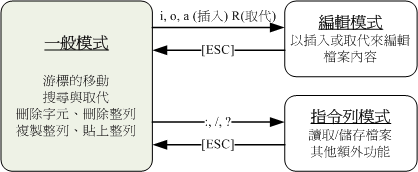
\includegraphics[scale=0.8]{pics/vi-mode} \\

\subsection{Basic knowledge}

\begin{itemize}
		\item go to github and download \linuxcommand{clone https://github.com/VundleVim/Vundle.vim.git ~/.vim/bundle/Vundle.vim}
		\item go to my github and download vimrc and change it to .vimrc
		\item go to my github and downlaod vim/after/ftplugin and rename to .vim/after/ftplugin
		\item go to my github and download vim/plugin/cscope\_map.vim and copy it to .vim directory.
		\item  

		\item \textbf{Rule1: Don't use arrow key any more. At first, you always want to use arrow key to move to right position in insert mode. That is not correct. Any time you want to move, just go back to normal mode, then use "hjkl" and other motion command.}I have disabled arrow key in my .vimrc file.

		\item \textbf{Rule2: Once you go to normal mode, you will have a lot of commands which you combines together to finish your task, 1)basic move, 2)fast move 3)delete+(motion,text ojbects) 4)visual,copy or move. After all necessary task,5)you can use i(I),a(A) o(O) to return back insert mode at right position.}

		\item \textbf{Rule3: I made some mapping in insertmode, but they are just for temporary action to avoid "Esc+one action+i". You should not think that is mainstream operation, just supplment methods. For example, if you want move cursor a lot, first go to normal mode, then use necessary commands,then come back to insert mode. That is better than <Alt+hjkl> in inser mode. If you just want to move one time, please use<Alt+h>.}

		\item \textbf{Rule4: Any time you click same key too many time, stop and google to see if you have better command or smart command, practice until you forget it. }

		\item \textbf{Rule5: But don't overdo it. Don't just focus on trick and plugin. If you can't find solution easily, just give up and focuse on your work, not tool}

		\item Esc is not in good position. You can use <C-$[$> to exit insert mode. You also can map jj to Esc. You also can map <Cap> to Esc. By now, my configuration support these three methods. 

		\item In terminal windows, in edit menu, you can see preference. You can "disable All menu access keys", In this way, you can use alt+f or alt+h key in your vim. 

		\item By now, I configure cursor in different shaps: 

		\item Use Vim, not vi. Vim is better than vi, previous figure is very important, you should click i to get insert mode. Then --insert will show on the bottom. If no --insert, that is common(NORMAL) mode. All the edit command(copy and paste) should be done under common mode. 

\item \linuxcommand{sudo apt-get install vim-gnome}, then use \linuxcommand{vim -g} will support mouse.  With mouse, you can click a position to move there. you also can drag mouse to select a block of text. It's easier to use it. 

\item :h s will give you detail information about each command. \verb=:h i_CTRL-W= will show a command "CTRL-W" represent in insert mode. "i\_" is insert mode. "v\_" is visual mode. And if you don't use any prefix, it represents all the command in the normal mode. There are two things worth mentioning: 1) Most commands in insert mode is combination key, such as CTRL-?. 2)In the help topic, you can see a lot of other optional insert commands around CTRL-W. You can extend your knowledge by learning other insert commands.

\item \linuxcommand{vim -v} will open read-only files. You also can use less, but less support motion command.

\item \verb=vim -version= will show you a lot if useful information. It will tell you if it support some mode or patch. For example, if you see +quickfix, It means that your vim support quickfix mode. If it shows -quickfix, maybe you need to recompile the whole vim.

\item .vimrc and .gvimrc are two important configure files, gvim  will read .vimrc first, and then read .gvimrc files.  You can use \verb=if has('gui_running')= to just configure for gvim, not vim in terminal. 

\item If you run vim in a terminal windows, terminal windows font and size will affect vim.  If you run gvim, You can configure vim font by add to .vimrc files.  

\item set LANGUAGE="en\_US.UTF-8" in /etc/rc.conf and LANG="en\_US.UTF-8" in /etc/locale.conf, then logged out and logged back in and it worked. My terminal displays unicode properly now. If don't have root right, set these two varaibles in your .cshrc or .bashrc file.

\item gvim's color is sharper than vim in terminal.  Maybe it use more colors than terminal.  

\item g and z don't use as any command in normal mode, so they are prefix as combinaiton command, such as zt,zb, gj, gk, gg. :help z and :help g will show you all the commands that sit behind these prefixes.

\item \linuxcommand{vim -u NONE} will laungh vim without laod .vimrc. It will help you if you have some troubles in your .vimrc file or you want to do some experiments. 
\end{itemize}

\section{basic command}
	\begin{itemize}
	\item Move, you should be able to move in both insert mode and normal mode. For some simple move, you should not leave insert mode, that means you can save some time.You need to use \verb!inoremap! to map to alt key, see next item.

	\item All <A-*> need to be use \verb!inoremap <A-t> <C-o>gg! command to map to a command in normal mode. In table, I just keep <A-*>, detail mapping can be seen in my .vimrc file. 

	\item there are few rules you need to follow:
			\begin{enumerate}
					\item Don't change any command in normal mode, when you use laptop or other compouter, when your mapping doesn't work well, you can return to normal mode to use these original commands in normal mode

					\item when you are mapping, you can refer the normal mode, such as <A-w> is move to next word, just like w command in normal mode.

					\item If you just want to have ONE action move or other operation, you don't need to leave insert mode, so mapping the mose used command in insert mode, by now, I mapping some move and editting command in insert mode. Detail can be seen in below table.

					\item By now, you can use Alt-char map some commands, and you also can use two captive lettes which don't use very often in our language. such as UU RR etc. 

					\item By now, on some computers, if you map alt-(char), It doesn't work very well. Sometimes, when you press it,it will go into the normal mode. I don't have time to investigate right now. 
			\end{enumerate}


	\begin{center}
		\begin{tabular}{p{0.33\textwidth}|p{0.33\textwidth}|p{0.33\textwidth}}
		\hline 
        move position & insert mode & normal mode \\

		\hline
		b/e of document &  <A-f>(begin)  & 1G(or gg) , G  \\

	    \hline 
		b/m/e of screen & <C-o>... & H, M, L \\

		\hline 
		pre/next para & <C-o>... &\{ \} \\

		\hline 

		pre/next sentence & <C-o>.. & $( )$ \\
		
		\hline 
		begin, end of line &<A-i>and <A-a> & (0 or \^{}) and (\$ or g\_)  \\
		

        \hline 
        Above, next line &<A-p> and <A-o> & O and o\\

	   	\hline 		
		next, previous word(begin) &<A-w>, <A-b>,<A-e>  & w, b\\   

	    \hline
	    next, previous word(end) & <C-o>.. & e, ge \\
 	
         \hline 		
         match parenthes & <C-o>... & \%   \\
         
         \hline match next character &<A-q>, <A-z>& fx, Fx \\
         
        \hline mark and return & <A-m> <A-n> & ma, then `a. \\
        
        \hline return to previous jump position & <C-o>... & <C-o> \\    
      				
		\hline
        search &<C-o>...  & / and ? \\

       \hline       
		previous and next word in cursor & <C-o>.. & \#, * \\

		\hline 
		All /first word in cursor(For C/C++) &  & $[I$, $[i$  \\ 

		\hline 
		will go to next line in wraped mode. & &  gj and gk \\
		\hline 

\end{tabular}
\end{center}
		\item h,j,k,l, w(W), e(E), b(B), \^ , \$ ,fx,tx, (,), \{ ..., gg. All these move command you can add number before them. For example, \verb=4f,= will jump to the fourth ,(comma) directly.    

\item jump lists basic:
		
\begin{enumerate}
		\item You need to know jump lists. there are single quote command, backtick command. One will jump to exact mark, Other will jump to mark line. They need follow a mark name.

		\item There are "G","/", "?", "n", "N","\%", "(", ")", "[[", "]]", "{", "}", ":s", ":tag", "L", "M", "H"

		\item "f F t T" will not go over multiline. It just search within one line. If you need to multiline search, you can use "/ ?"

		\item All jump command will record in jump list; You can use :ju to see a list of it.

		\item Double single quote and double backtick will toggle current and previous jump. Double backtick will come back excat position. Double single quote will come back previous line position.

		\item :ju will show jump list. Then you can use <C-o> and <C-i> to navigate the jump list. 

		\item fx command, then ; and , will repeat forward and backward command, Just like n and N in / and ? command.

		\item gi or `. will return your last edited position. 
\end{enumerate}

\item Below are some edit commands:
\begin{center}
		\begin{tabular}{p{0.33\textwidth}|p{0.33\textwidth}|p{0.33\textwidth}}
		\hline
		delete & insert mode & normal mode\\

   	    \hline 
		delete previous character & backspace,<C-h> & hx(move then x)  \\
		
	
		\hline 
		delete and replace current character & <A-x> & x , s , r\{char\}  \\
	
		\hline 
		delete word to end & <A-c> &dw or cw  \\
		
		\hline 
		delete word to begin & <C-w> &db or cb  \\

		\hline 
		delete current word &<A-b>,then <A-c> & daw or daW \\
		
		\hline 
		delete line to end & <A-v> & d\$ or c\$  \\
		
		\hline 
		delete line to begin & <C-u> & d\^{} or c\^{}  \\
		
		\hline 
		delete current line & <A-d> & dd cc \\

       \hline
	   replace in current line &<C-o>.. & :s/old/new/g(c) \\

	   \hline
		indent and unindent & <C-t> <C-d> & >> and << \\

	   \hline 
	   Join next line & <C-o>.. & J \\ 

	   \hline 
		swap line with next &<C-o>.. & ddp \\
	
		\hline 
	   replace in whole file &<C-o>.. & :\%s/old/new/g(c) \\

		\hline 
		undo and redo & u and . (ctrl+r)  & <A-g> \\ 
		
				\end{tabular}
	\end{center}
	
\item tricks about edit command: 
\begin{enumerate}

				\item  Edit commands "d,c,y", c go to insert mode. y keep contents. All edit command "d,c,y" can follow motion, it give edit command a "operator scope". For example, "d2w" will delete next two words. "d3j" will delete next 3 lines. "ct;" will delete every thing until ";", it's very useful for C++ language. 

			\item 3dd and 2dw   \& support number+command means how many times you will perform this command.

				\item x stay in normal mode, s go into insert mode, r need to follow a letter and stay in normal mode too.
				
				\item \textbf{Usually, You can delete a character(x),change a character(r) delete a word(diw), delete to b/e or delete line(dd). Even delete next few lines (d3j). You also can insert an character <leader>i and <leader>a in normal mode. }  
				
				\item All the edit command "d,c,y" can follow motion, at the same time, It also can follow text object, such as "aw" and "iw". A list of text objects can be see below.  You can use \verb=di"= to delete all the contents inside of a pair of double quotes. You also can use \verb=da"= to delete all the contents plus a pair of double quotes.There are 11 groups common used text objects which I introduced in previous section. 
						
				\item command v also can follow motion and text objects. It can give me a tip. If you are not sure what you will delete, you can use v command to highlight, if highlight is not what you expect, you can Esc, and adjust you motion or text object, until you get what you expect. 

				\item ggyG will select all contents in a file. such as Ctrl+A and Ctrl+C 

			\item "ddp" swap lines. In fact, it is two commands, "dd" and "p". If you understand it. you can know "xp" is swap character. And "dawp" is swaping word.

			\item "J" can be use to delete empty line below.
	\end{enumerate}

\item scroll command, scroll window, but cursor will stay in the same position.
		\begin{center}
 \begin{tabular}{p{0.33\textwidth}|p{0.33\textwidth}|p{0.33\textwidth}}
        \hline
        scroll one  page &  <A-t> and <A-y>  & ctrl+b and  ctrl+f    \\
        
        \hline 		  
        scroll one line &  <A-u> and <A-r>  & ctrl+e and ctrl+y \\
        
         \hline 		  
        move cursor to m/t/b & <C-o>...    & zz zt zb \\

    \end{tabular}
\end{center}
 
\item move and window

\begin{center}
   
  \begin{tabular}{c|c|c}
   \hline
		move & insert mode & normal mode \\
		
\hline 
		switch window & <C-c> &  Ctrl + w\{h,j,k,l\}\\
				
		\hline 
		split window & <C-o>,then :sp  &  Ctrl + ws\\
		
		\hline 
		close a window & <C-x> & Ctrl + wq\\
		
		\hline
		split window vertically	&   & :vsp \\ 

			\end{tabular}
	\end{center}

\item move  buffer

\begin{center}
\begin{tabular}{p{0.33\textwidth}|p{0.2\textwidth}|p{0.33\textwidth}}
   \hline
		Action & insert mode & normal mode \\
		
\hline 
		edit a file in a new buffer & &  :e file\\
				
		\hline 
		next, previous buffer & RR &  :bn :bp , <C-\^{}> \\
		
        \hline 
		go to number buffer &<C-o>.. &  :b num \\		
		
		\hline 
		delete a buffer & & :bd \\
		
		\hline 
		list all open buffers & & :ls\\
		
		\hline
		open a file in a new buffer and split window
	 & <C-o>..& :sp :vsp \\
		
			\end{tabular}
	\end{center}

	\begin{enumerate}
			\item Closing windows is different with deleting buffer.When you use :bd command. It will close the windows too. If you want to just close buffer. You shold use :bn to switch to another buffer, then use :ls to know the buffe number which you want to close, in the end. use :bd numclose to close it background without close current windows.
				\item use :ls! command will show all the buffers. Such as Nerdtree buffer, VimtexToc buffer. To reload buffer into certain windows. 

			\item bd will close current buffer, you can follow number to close specific buffer. You also can use :bd+space+tab will list all the avaible buffers.
			\item Any time you want to switch buffer or open new buffer, save current buffer first.
			\item ":e" will open buffer in current window. If you want to open in a different window, you can use "sp file" or "vsp file".
	\end{enumerate}

    \item commands in visual :
    
    \begin{center}
        \begin{tabular}{c|c}
				\hline
		v, Ctrl-v  & being select\\

		\hline 
		d, y & copy and delete\\

		\hline
		<,> & indent left,right\\

		\hline
		V, yy & select, copy the whole line  \\

		\hline
		gv & reselect previous select
		
			\end{tabular}
	\end{center}

	\begin{enumerate}
			\item Using v to exit select mode is faster than Esc. 
			\item <,> will exit select mode, gv will select it again. 
	\end{enumerate}					
	
	\item format command : Other reformat tricks can be found in next section "Programmer tips" 
 \begin{center}
        \begin{tabular}{c|c}
		\hline 
		=, =\% & format, format\verb={..}=\\

		\hline
		== & format current line \\ 
		\hline 
		15G=25G & will reformat from 15 to 25 lines
		
			\end{tabular}
	\end{center}
		\item In Vim, there are three clips:
				\begin{enumerate}
						\item normal clip, You only can use mouse to select(It will add line number into your selection), then in insert mode, right-click mouse to popup menue, select paste; Or shift+insert. \textbf{Don't use Ctrl+C and Ctrl+v, and must do it in insert mode, or all you content will be input as command in the normal mode, It's dangerous}
						\item xclip, Use mouse middle-button to past in Vim.\textbf{Must in insert mode}
						\item vim own clip, use y and p command. \textbf{Must in normal mode}
						\item :reg will show your list of register."0 will always have the content of the latest yank, and the others will have last 9 deleted text, being "1 the newest, and "9 the oldest.
						\item The contents of a register can be pasted while in insert mode: type Ctrl-r then a character that identifies the register. For example, Ctrl-r then " pastes from the default register
						\item Use \linuxcommand{vim --version} to see if vim has been compiled with clipboard, If there is + symbol before it. You can use "+y and "+p to copy and past selection to system clipboard. If not, Just use mouse middle-button.
						\item Sometimes, when you copy source code from brower, then use shift+insert to paste it, The format will be messed. You should use shift+mouse to select and copy content to xclip. Then in your vim, 1) move your cursor to insert position, 2) in normal mode run \verb=:r!xclip -o<CR>=, it will paste according to right format. Don't use normal clip and xclip in insert mode.
						\item Add key map to .vimrc, detail can be found in .vimrc file.By now, I map it to F6 and F7. 


				\end{enumerate}

\end{itemize}

\section{Plug in}
\subsection{vundle}
\begin{itemize}
		\item About vundle usage, I have added a bookmark to evernote. First you need run "git clone https://github.com/VundleVim/Vundle.vim.git ~/.vim/bundle/Vundle.vim", then just need to edit .vimrc file.  

\item When you have vundle installed, you can edit .vimrc to install others plugin. By now, I have backup my .vimrc file. When you transfer to other computer, you can use it directly. 
		\item You can google "vim awsome". It introduce a lot of vim plugins. By now, what I installed can be found in .vimrc file. 
		\end{itemize}

\subsection{solarized}
\begin{itemize}
	\item vim-colors-solarized, it can be only used in vim in terminal, It only support 16 color. You need to go to  vim "color scheme test c website" (add it evernote) and select you favorite scheme. and then download it. put it in .vim/bundle/vim-colors-solarized/colors directory. Then you can modify your .vimrc.
	
\begin{verbatim}
if has('gui_running')
colorscheme blacklight
else
colorscheme solarized
endif 
\end{verbatim}
	\item When you use solarized plug in(theme), you have to change the terminal. For some new version gnome terminal, you can see terminal->preferences->profiles->color tab, there is solarized dark option in "text and backgroud color", and solarized option in "build in scheme in palette", just select it.

    \item When you have old terminal, There are two options, for some old gnome
        terminal, there are no import color option, you can download
        Anthony25/gnome-terminal-colors-solarized in a temp directory, and then
        come to this directory and run .install. You need to first add an solarized profile, then the application will ask if which profile you like to overwrite, select solarized profile, you can keep you original default unmodified. Then you can select your solarized profile, the color will be set properly. 

\item If some keyword highlight background color is not correct, you need add \verb!set t_Co=16! to your .vimrc. 

		\item For mac, you can download
        tomislav/osx-terminal.app-colors-solarized(I haven't tried it yet). Or
        you can download git:altercation/solarized. there is directory \verb!osx-terminal.app-colors-solarized/!, you can import *.termnial file in
        your mac terminal preference color. That is all.
\end{itemize}

\subsection{vim-airline} 
\begin{itemize}
\item For vim-airline,  First, you need to download Powerline font(github), then ./install.sh. because vim in termial use terminal font, so you should expect it have beautiful interface. It will install font to .local/share/font. Then you should add below to .vimrc.  Put statement in if, or It will make vim in terminal a little bit ugly. 
\begin{verbatim}
if has('gui_running')
set guifont=Literation\ Mono\ Powerline\ 12   
let g:airline_powerline_fonts = 1
endif
\end{verbatim}
\item You can go to "https://github.com/powerline/fonts" download font package. Then extract it. Go into the directory, then run ./install.py.  All the font will be installed in HOME/.local/share/fonts. Then you go to your HOME directory. build a link. "ln -s HOME/.local/share/fonts .fonts". Then you gnome-terminal preferecne window will show Powerline fonts. Slect "Literation Mono Powerline". Building link is very important step for gnome-terminal. 
\end{itemize}


\subsection{NerdTree}
\begin{itemize}
		
		\item \textbf{Use ctrl+N to toggle nerdtree window}, then Ctrl+C change window, once you are in nerdtree window, you can use all motion command in normal mode to move your cursor. You also can change to visual mode and use 'y' to copy a file name and paste it back to your main editor file.  

		\item shift+i will show or hide hidden file
		\item When in the NERDTree window, press 'm'; you should see a menu at the bottom. Type in 'a' for add childnode. Now input the directory you want to create, making sure to add a '/' at the end, otherwise the script would create a file.
		\item In the NERDTree window, you can press 'm' and 'l', then you will get whole directory informaiton. Then you can use mouse to copy it and paste it back to your main edited file.
		\item When you are in the Nerd window, you can press Enter to open in current windows. "s" will open in vsplit window, "i" will open in a split window, If you forget, press "?" to toggle to show all the useful commands.

		\item For some very deep file, you can use :Bookmark bm. Then "B" will show all the Bookmark table. Then you can navigate Bookmark table to open a bookmark file.
		\item You can use "u" to jump up one level in directory tree. Or use "C" to change current directory as tree root."r" will refresh the directory.
		\item By now, preview will open a new buffer inside vim. So this feature is not what it really like. There are some solutions, but I don't want to try them right now.

		\item use p to jump to parent folder position, and .. go up level
\end{itemize}

\subsection{Ctrlp}
\begin{itemize}
\item use ctrl+p to invoke ctrlp plugin, Don't use :CtrlP command  \\ 
\begin{tabular}{|p{0.25\textwidth}|p{0.75\textwidth}|}
\hline 
ctrl+f,b  & cycle between modes \\ 
\hline 
ctrl+r & switch regex mode  \\ 
\hline 
ctrl+d & switch to filename search instead of full path \\ 
\hline 
ctrl+o, t or x & open, open file in new tab or in new split \\ 
\hline 
ctrl+z  & mark and unmark files \\ 
\hline 
\end{tabular} 
\item CtrlP will open "current working directory" in vim. You can use :cd directory to change "working directory". You also can input .. to go up parent directory. Default, CtrlP also look for .git as a flag of "Whole project". You can custom your favorite setting according to your context.

\item CtrlP also provide "most recent files" function.

\item \textbf{With Ctrlp and NerdTree, vim has powerful tool to deal with files and directory. You can navigate file system structure by Nerd, add mark by Nerd, or search them quick by CtrlP}
\end{itemize}



\subsection{Vimtex}
\begin{itemize}
		\item Vimtex is lightweight plugin for Vim. I didn't use compile ability right now. 
		\item Vim tex provide anothe text objects. Such as "ae ie", "ac ic" and "ad id". 
		\item By now, I map F3 to :VimtexTocToggle.
		\item ]] in insert mode finish enviroment automatically.
		\item [[ ]] command navigate by section.
		\item (cd)*(se sc sd) six commands. 
\begin{verbatim}
1)\begin{aaabbb}
ac is "\begin{aaabbb}"
ic is "begin"
dsc will delete "\begin{}" and left aaabbb

ae is whole enviroment
ie is inside enviroment
dse will delete "\begin{}" and "\end{}" 
\end{verbatim}
	\item By now, I don't delimiter, it used mainly for math equation. So I don't use "ad id" and "dsd" very often. 
			\end{itemize}

\subsection{Emmet}
\begin{itemize}
		\item <C-y>, is trigger key in Emmet. I map "hh" to expand abbreviation.

		\item Below is simple table, detail can be google by"emmet abbreviations syntax". Abbreviation is the most important topic in Emmet. Besides, it, It provide other useful command. 

\begin{tabular}{p{0.25\textwidth}|p{0.75\textwidth}}
\hline 
html:5  & whole page \\ 
\hline 
>,+,\^{} & child,sidling, parent  \\ 
\hline 
* &how many times output \\
\hline
div\#id, div.class & with id and class to a tag \\

\hline 
\$ & will attach number with elemental attribute name   \\

\hline
text \{ \} & add text to element \\
\hline
\end{tabular}

\item An example, type \verb=div>p#foo$*3>a=, The <C-y>, 
 <div>
       <p id="foo1">
		   <a href=""></a>
	   </p>
	   <p id="foo2">
		   <a href=""></a>
	   </p>
	   <p id="foo3">
		   <a href=""></a>
	   </p>
</div>

\item Some directly edit commands. \\

\begin{tabular}{p{0.25\textwidth}|p{0.75\textwidth}}
\hline 
<c-y>+k  & remove a Tags pair and content inside \\

\hline 
<c-y+d,D & Balance tag outward and inward  \\

\hline 
<c-y>+a & move to URL, add anchor to it \\

\hline
<c-y>+/ & toggle comment \\

\hline 
<c-y>+i & In image tag, refresh image \\

\hline
ctrl+n,N & move to next avaible position \\
\hline 
\end{tabular}

\item This tutorial is very simple, website give you detail examples, you can learn it when you work on html pages. 

\item You can type p, then type hh, It will expand <p></p> and insert cursor will be in the middle. 

\item For some exist test, first select, then type <C-y>,, It will move curser to bottom to wait for you input tag.You just need input "h1", don't need to input "<h1>". Emmet will add < > for you automaticlly. If you use surrounding, select, and shift-s. input "<h1>". 


\end{itemize}

\subsection{Easy motion}
\begin{itemize}
		\item Jump to word, use <leader><learder>w,b,W,B,e,E,ge,gE. 
		\item For multi-line, use <leader><leader>j,k.  
		\item :help easymotion.txt give you detail information.
\end{itemize}

\subsection{Surround}
\begin{itemize}
		\item There are three main actions. delete(ds), change(cs) or add surrounds(ys)

		\item When you use delete or change, you should put your cursor inside a pair of surrounds.\\

		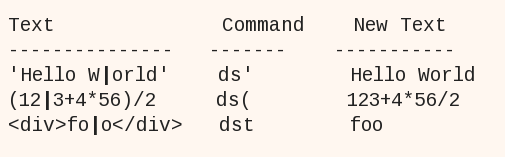
\includegraphics[scale=0.4]{pics/surround1.png} \\

	\item below is change command list: \\

	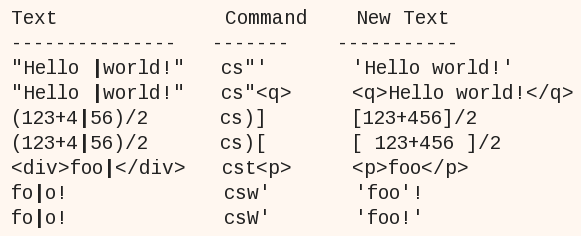
\includegraphics[scale=0.4]{pics/surround2.png} \\
		
		\item Surroundings can be added with the same "cs" command, which takes a surrounding target, or with the "ys" command that takes a valid vim motion. \\
			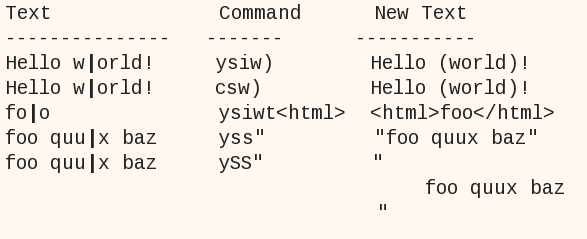
\includegraphics[scale=0.4]{pics/surround3.png} \\
	   
	   \item You can use csw" or ysiw" to add surrounds. ys can follow a valid vim motion. Such as ys3w<p> will add <p>word1 word2 word3</p>

	   \item In Visual mode, press <S-s> (captive S). Then input a surround that you want to add. Don't sue lower case "s". 
	   \item You need install repeat plugin too. For example: there is text "<p1><p2>word</p2><p1>". You put cursor inside word. Then you can use dst. Then press . It will delete pair of <p1> and <P2>
	    
	    \item Surrounds are useful for edit html doc. It's overlap with Emmet. For example. In visual mode. \verb=<C-y>,= will trigger expand mode in Emmet. Then input <h1>. Or you can use <S-s>, then input <h1>. It will add a pair of <h1> 
	    \item For a single line. You can use yss command. It's better than Emmet. In Emmet, you have to visual select this line first.  
\end{itemize}

\subsection{Repeat}
\begin{itemize}
\item . only repeat edit command in norm mode. And only for these native edit command. It will not repeat move command

\item move command are most single character, So I don't need to use . to repeat it. If you like, there is plugin for it. 

\item For some customized edit command, such as Surrounds below. native . command will not support it. So, I need to repeat vim plugin installed. 
\end{itemize}

\subsection{match it}
\begin{itemize}
		\item It's old plugin, so maybe it will not work very well, Don't expect it too much.
		\item It support <p> </p> jump and /begin /end jump.
		\item It don't need if..else if.... jump. But you can build .vim/after/plugin/c.vim and cpp.vim. and add below to it. And it will support if..else if... else jump and switch...case. default. jump
		\item g\% will jump backward. 
\begin{verbatim}
let b:match_words= '\%(\<else\s\+\)\@<!\<if\>:\<else\s\+if\>:\<else\%(\s\+if\)\@!\>,' . '\<switch\>:\<case\>:\<default\>'
\end{verbatim}

	\item There is another python matchit plugin. It support for(while)...break(continue). if..elif..else, and try..except..finally jump.   
\end{itemize}

\section{Text Block}

\subsection{text object}
\begin{itemize}
		\item Common text objects in vim. 
\begin{verbatim}
aw		a word (with white space)
iw		inner word
aW		a WORD (with white space)
iW		inner WORD
as		a sentence (with white space)
is		inner sentence
ap		a paragraph (with white space)
ip		inner paragraph
ab		a () block (with parenthesis)
ib		inner () block
aB		a {} block (with braces)
iB		inner {} block
at		a <tag> </tag> block (with tags)
it		inner <tag> </tag> block
a<		a <> block (with <>)
i<		inner <> block
a[		a [] block (with [])
i[		inner [] block
a"		a double quoted string (with quotes)
i"		inner double quoted string
a'		a single quoted string (with quotes)
i'		inner simple quoted string
a`		a string in backticks (with backticks)
i`		inner string in backticks
\end{verbatim}
\item There are "a,i" two big categories. There are "w,s,p", "b,B $[$", and "double quote,single quote, backticks". Inaddtion, There is extra "t,<", Just remember 11 group.You can use them in the "d,c,y"commands. Don't forget you can use v command to see if scope of these text objects in your text.  

\end{itemize}



\begin{tabular}{p{0.15\textwidth}|p{0.23\textwidth}|p{0.63\textwidth}}
\hline 
type & text object & surround \\

\hline 
",',`  & (a,i)(",',`) & f"(jump), cs"(, ds" \\

\hline 
\verb=(,{,[= & (a,i)(b,B,$[$) & \%(jump) ds(,cs("  \\

\hline 
<p> head </p> & (a,i)(t,<) & \%(matchit), dst, cst<h1>, 1) phh(Emmet) 2)select,S,<p>(Sround) 3)select,<C-y>,p(Emmet) \\

\hline
/begin ../end & (a,i)(e,c) & \%(matchit), dse, dsc \\

\hline 
w,s,p & (a,i)(w,W,s,p) & Add surrounds: csw", csW", ysiw" yss".  \\

\hline 
\end{tabular}

\section{Programmer tips}
\subsection{Basic}
\begin{itemize}
 	\item In .vimrc file add below for c++ programming 
\begin{verbatim} 
set tabstop=3
set shiftwidth=3
set number	
\end{verbatim}
\item Build a IDE-like Vim, You need below plugins:
		\begin{enumerate}
				\item File explore: NerdTree and CtrlP
				\item Tag jump: tagbar, cscope and easyGrep, gD command and Ctrl+](need tags file),Ctrl+T return.
				\item Error jump: quickfix.
				\item Syntax: syntastic plugin(For python and C++, YCM will use Syntax show syntastic errors)
				\item Autocomplete: SuperTab, Vim-snippet, Ycm, Ctrl+p
				\item Debug: pyclewn
				\item Comment: Nerdcomment
				\item Fold: For C/C++, just :set foldmethod=syntax, For python language, use simpylFold plugin 
		\end{enumerate}
		
		\item Python indent show plugin is <leader>ig. You can change its color if you dislike default configuration. 				
\item Why jumping to brace is so important? First, use previous commands to jump to open brace. Then \verb!=\%! will format the matched scope. \verb=v\%= will select the whole scope.  After you select, you can input = command to reformat. 
		
\item Reformat will perform action according to the previous lines indents. So before reformat, you can use == reformat the previous line of code to right indent.
 	
	 \item ctrl+v will invoke visual-block, you can decrease indent of block or delete a block of comments. 
	 
			 \begin{enumerate}
					 \item ctrl+v, then select block of comment source code 
					 \item don't press Esc, press I (capital i) 
					 \item input // 
					 \item press Esc, then, all the block will be commented.
			   \end{enumerate}
	 \item set number; syntax on and set ai;  whenever you hit Enter to start typing on the next line, vim automatically will indent to the same amount as the previous line.

\end{itemize}

\subsection{Fold}
\begin{itemize}
	\item For fold C/C++ correctly, write Big bracket after class, function and if.. statement, and keep them in the same line. \textbf{I need to use this style all the time.} I didn't use fold function very often. 

		\item In vim ,there are different fold methods, and you can't combine them together.  The most useful Syntax, And if you want to use zf command, you have to change it to "manual" method. 
				
		\item fold commands are below, they are VIM commands, not plugin command.

\begin{tabular}{|c|c|}
\hline 
\textbf{key} & \textbf{action} \\ 
\hline 
za, zo, zc & toggle, open, close \\ 
\hline 
zj,zk  & jump to previous and next fold\\ 
\hline
zM, zR & Close , Open all \\
\hline 
$[$z, $]$z & move to the start and end fold \\
\hline 
zf\string & fold to string \\

\hline 
 
\end{tabular} 

\end{itemize}

\subsection{Syntastic}
\begin{itemize}
		\item :Errors to open error windows.  

		\item Everytime when you save file, syntax error will listed on left side.

		\item You can use :lne to jump to next Syntastic error, use :lclose to close Errors windows. They don't need to  switch to error windows. 
				
		\item There are two checker for latex, one is chktex, you can download and install it from source code. The other is lacheck. lacheck will not ignore text in lstlising enviorment, and it will report a lot of errors. It's annoying. chetex can ignore content in lstlisting enviorment.

		\item You can goto tex document directory, you can build a .chktexrc file and add below to it. 

		\item For Syntax error use :Errors, it open location list.  For compile error, use quickfix mode, It use quickfix window.   nowarn use to suppress some unnessary warning message.
\begin{verbatim}
CmdLine{
--nowarn 1
}

VerbEnvir{  verbatim comment listing verbatimtab rawhtml errexam picture texdraw
  filecontents pgfpicture tikzpicture minted
}
\end{verbatim} 

\item You can add \verb!let g:syntastic_tex_checkers=['chktex']! to tell Syntastic use chktex to check latex.

\item For latex document, there are a lot of unimportant error, You need to supress them. When you use lacheck, you can't suppress warning. But you can add tex.vim file to after/ftplugin to deal with some tex type file. In this file, you can add let g:syntastic\_quiet\_messages to it, detail can be seen this file.


\item chktex doesn't check unmatch big brace, but lacheck will not ignore lstlisting env. \textbf{So, They are not good tool for latex check, just a refence, not perfect at all, Don't spend time on them}.

\item default use chktex, after write, jump to Errors windows and search "error", If there is no error, You can use lachek in you command line to look for unmatch brace error if you document doesn't have lstlisting env. That is all.
\item \textbf{For Cpp latex document, use chktex, in other document, use lacheck and don't use lstlisting enviroment}

\item For python language, you need to install flake8. You can use \linuxcommand{pip install --user flake8} to install it. It will install it in ./local/bin directory. 

\item For html language, You need install tidy, By now, I download it from github and use cmake to build it. detail can be found in build document. 

\item My web use a lot php file. So You need to add this line to .vimrc. So when you edit .php file, when you save it. It will use tidy to check all the html content in php file.
\begin{verbatie}
let g:syntastic_filetype_map = { "php": "html" }
\end{verbatie}

\item :SyntasticInfo will show some helpful informaiton, when syntastic doesn't work, you can run this command to see some detail. 

\item Syntastic use clang to check errors in C/C++ language. 

\end{itemize}
\subsection{Code navigation}
\begin{itemize}
	\item gD, go to the func or variable defination. It's just jump the first appearance in the current file. It has no any semantic. Another otpion is Ctrl+], it's just like :tag command. It will need you have tags file produced by ctags command. For example, you can use ctags a.cpp to produce tags file, then in you vim, you can use Ctrl+]. The problem is by now, ctags doesn't produce local varaible inside a function.  This problem can be resolved by easyGrep partly.

	\item  Program motion:
\begin{enumerate}
 	\item C/C++ jump bracket:
%\begin{lstlisting}[frame=single, language=c++]
\begin{verbatim}
fun()
{"[["
   ...
}"[]"

main()
{"[["
   {"2[{"
	 {"[{" 
	   {"?{"
	   }
	   {"F{"     } *
}
{"]["
.....
}"]]"
%\end{lstlisting}
\end{verbatim}
\begin{enumerate}
		\item * is your position
		\item \verb=[[,[],][,]]= First is directory, second is opening or closing brace. They just jump to the first column
		\item Find match open brace, you should use f/F or /or? command. 
		\item \verb=[{ or ]}= will jump backward unmatch braces. 
		\item \verb=[( or ])= has same usage.
\end{enumerate}

\item \% can be used jump brace, with Matchit, You can use it jump if else in C and try except in python. You need to another file to support it, detail can be found MatchIt section. 

\item Visual Mark is also a good plug in, usage is very simple, mm visual mark, F2 and shift F2 navigate.

\item Tagbar support python and C at the same time. Cscope only support C/C++.

\item EasyGrep is also a good plugin, detail can be found in below plugin part. 1) Just like cscope, it can be used for python file and produce a list reference position, 2) It support replace mode, and it's very helpful for refactory.
\end{enumerate}
\item \textbf{Tagbar give yo global scope function name and variabel, but It will not give you local variable. It support C/C++ and python file}

\item \textbf{easyGrep only support multi file search, If you need loca file, you can use lvim, It will show a list result in location window, you can use lopen, lne, lpr, lclose command}

\item \textbf{cscope support a little syntastic analystic, Anytime when you modify files, you need to produce new cscope.out file and it doesn't support python language}

\end{itemize}

\subsubsection{EasyGrep}
\begin{itemize}
		\item add let g:EasyGrepMode = 2 to .vimrc. It will only look for the same kind of file extension. 

		\item <leader>vv, look for word,  <leader>vV match whole word. It will show all the result below the window, just like quickfix mode
		\item You can use all :cn :cp command in quickfix window to move. 

		\item <leader>va will add find to current quickfix list. 

		\item The mose useful feature is <leader>vr, it will find all match word, and ask you if you like replace it with certain target word. It's useful to refactory you code. 
\end{itemize}

\subsubsection{Tagbar}
\begin{itemize}
\item Tagbar can show all the tag(function, variable and macro...) in a different windows. It's better than taglist. But you need to install Exuberant ctags(Use archive manager in mint to install, It's very easy)

\item common used shortcut.	\\	
\begin{tabular}{|p{0.35\textwidth}|p{0.55\textwidth}|}
\hline 
s in tag window & change order \\ 
\hline 
space in tag window & show tag prototype in command line  \\ 
\hline 
- and + in tag window & fold and unfold \\ 
\hline 
q in tag window & quit tag window \\ 
\hline 
\end{tabular}
\item In Tagbar windows, just like NerdTree window. Press ? will show your basic key shortcut. 
\item By now, Tagbar use CTag as support. Tagbar just show tag file produced by CTag. CTag doesn't support to produce variable inside function. Maybe new version CTag will support it. 
\item You don't need run any command. Just add it to .vimrc or use :TagbarToggle directly. By now, I mapped it to F8
\item Ctag default does't parse the local varaible inside function, You can turn on it in ctags, but it wil make tag file much bigger, and most of time, If you can keep your function shorter, you will not need list all local variable inside a fuction in the tagbar winodws. So default this option is disable. 
\item Usually, you can keep tagbar window open, it can help you navigate your source code more quickly. 
\end{itemize}

\subsubsection{Cscope}
\begin{itemize}

\item cscope is another application which you can navigate tags in source code. 
\item In vim, you don't need any plugin. Just like quickfix. You need to use vim --version to see if there is +cscope in output. 

\item Run \verb=cscope -Rbq= in you directory which include C source code, it will output three files. One is cscope.out. It's basic index file. 

\item Default, cscope only scan C file. If you want it to scan C++ file. Build \textbf{cscope.files} and add all your C++ file into it. Or you can use find command to write c++ file name into this cscope.files.

\item :cs add, then press tab, It will loop previous files. select \textbf{cscope.out}, then enter.

\item Use below commands to look for tags \verb=:cs find= 
\item <C-R> and <C-W> you can paste current word into command line. <C-R>" paste you just yank content. Pay attention to: R and W are captive letters.
  
\begin{tabular}{p{0.1\textwidth}|p{0.85\textwidth}}
\hline 
's'  & symbol: find all references to the token under cursor \\
\hline 
'g'  & global: find global definition(s) of the token under cursor \\
\hline 
'c'  & calls:  find all calls to the function name under cursor \\
\hline 
't'  & text:   find all instances of the text under cursor \\
\hline 
'e'  & egrep:  egrep search for the word under cursor \\
\hline 
'f'  & file:   open the filename under cursor \\
\hline 
'i'  & includes: find files that include the filename under cursor \\
\hline 
'd' &  called: find functions that function under cursor calls \\
\hline
\end{tabular}
\item You can use Tagbar and cscope at the same time. It will help you to jump to tags very quickly. 	

\item Download cscope\_map.vim, and put it in the .vim/plugin directory. Maybe you need comment line 42 because it will add cscope.out file twice, it will cause error. This plugin will help you to extract word under cursor. You can use Ctrl+\ then press s,g,c,d,t.. Use it in the normal mode. 

\item Add \verb!set cscopequickfix=s-,c-,d-,i-,t-,e-! to cscope\_map.vim, It will show multi result in quickfix window. Then you can use :cw window to open it, and :cn and :cp to navigate it. Default window will close automatically when you press enter, I don't like it. 
\end{itemize}

\subsection{Other Edit}

\subsubsection{NerdCommenter}
\begin{itemize}
		\item Main commands lists:  

\begin{tabular}{p{0.6\textwidth}|p{0.4\textwidth}}
		\hline 
		[count]<leader>cc & Comment out \\
		\hline 
		[count]<leader>cu & UnComment out \\
		\hline 
		[count]<leader>c<space> & Toggle Comment \\
		\hline
		[count]<leader>cn & Force nest comment \\
\end{tabular}
\item You can select or use number before these command to give a scope. 
\end{itemize}

\subsubsection{Visual-Mark}
\begin{itemize}
		\item Ctrl+F2 only work in gvim, In vim use mm.
		\item In visualmark.vim, there is space after keymap mm, So everytime when you press mm, It will fold document. you need to go to visualmark.vim and delete Space character after mm keymap.
		\item How did I find this? you can use :nmap to found all the current command list. \textbf{This is very useful when you found there is something wrong with one command.}
\end{itemize}

\subsection{quickFix}
\begin{itemize}
\item Default makeprg is "make", but you can use change it to:
\begin{verbatim}
:set makeprg=gcc\ -Wall\ -ohello\ hello.c 
\end{verbatim}

Add \verb=\= before space. In this way, you don't need Makefile in this directory.
\item First use :cw open quickfix window. Then in this windows, you can use :cn and :cp jump. The cursor will jump in code window  too. 
\item \textbf{You don't need install any Plugin. But For any C++ project, You should build a make file.} Detail can be found in the next chapter.  You can save a make template for simple C++ project. 
\begin{tabular}{c|c}
\hline
cc  &    show error detail \\
\hline
cp  &     pre error \\ 
\hline
cn &   next error\\ 
\hline
cl &     show all error\\
\hline
cw &    If there is error, open quick fix \\ 
\end{tabular}
\end{itemize}

\subsection{pyclewn}
\begin{itemize}
		\item If you system has pip, you can use pip intall, if you don't have root right, with --user, detail can be found google "pyclewn install".It's not installed by vundle. 

\item vimgdb is old, Don't use it anymore.

\item Open a new terminal, run command tty to know terminal name.

\item In you gdb, use tty command to redirect stdout and stderr to new terminal

\item In your new terminal, use Sleep(9999). Then you can use new terminal as input. 
\end{itemize}

\subsection{AutoComplete}
\subsubsection{YoucompleteMe}

\begin{itemize}
\item YoucompleteMe popup windows has bad color scheme. you can add two statments in .vimrc to change it. But by now, new version YCM seems to have better color. If you think default color is ok, You don't need to use below statements. 
\begin{verbatim}
highlight Pmenu ctermfg=Bule ctermbg=White guifg=#000000 guibg=#66cc66
highlight PmenuSel ctermfg=White ctermbg=Blue guifg=#ffffff guibg=#5cadff
\end{verbatim}

\item By now, YoucompleteMe support C/C++, python. For C/C++, you need install clang, For support python, you need to install Jedi, You can use pip install --user Jedi. It will install a package in .local/lib/python2.7/site-package.(It's not execuate binary)

\item Ycm has identify autocomplete, and semantic autocomplete. 
\begin{verbatim}
let g:ycm_auto_trigger = 1
let g:ycm_min_num_of_chars_for_completion = 99                 "
let g:ycm_key_invoke_completion = '<C-a>'
nnoremap <leader>jd :YcmCompleter GoToDefinitionElseDeclaration<CR>
\end{verbatim}
It will turn on two qutocomplete, min\_num option will turn off identify, but you can use <C-a> to trigger identify autocomplete manually. Semantic autocomplete will triggered by ., -> and ::

\item Use ctrl+n and ctrl+p will navigate options, Once select, input at the same time, Esc means that you will accept it. If you don't want to select, navigate to select Nothing. 

\item "Ycm\_show\_diagnostics\_ui = 1" will disable Syntastic check for C/C++, So :Errors will not work for C/C++. But when you save, a error tag will appear in vim gutter, when you move to this line, a error desrciption will appear in the command line. 

\item When you select a option, a preview window will popup in the upper part. 

\item If you install YoucompleteMe, You can install Syntastic, YCM will use Syntastic to show some error message.   

\item For autocomplete, You can use SuperTab, Vim-Snippet, Ctrl+P and YCM four plugin. The previous three use Tab, and fourth use . and -> .

\item You need to compile YCM to complete ycm\_core.so file. Git has install explanation. If you system is too old, you should upgrade your system first. I recommend that you use new version Ubuntu or xubuntu, Then download llvm pre-build binary from llvm.org to get libclang.so. \textbf{Don't try to compile YCM on old system. It has a lot of random problem if you config your own G++ compiler}

\item After you compile, you need .ycm\_extra\_conf.py file. I have kept it and upload to google drive.

\item You need to add some include path directory into .ycm\_extra\_conf.py file.\verb=g++ -E -x c++ - -v < /dev/null=. It will show all the include path. Then you can modify .ycm\_extra\_conf.py file.

\item For YCM-generator, It's easy to use, jut go to .vim/bundle/YCM-Generator, then run config\_gen.py pro\_dir. The pro\_dir should includes Makefile file in it.  It will run make clean first, then dry-run make to collect all the compiler flag. It remind me the understand buildspy. 

\item let g:ycm\_auto\_trigger = 0. When you type any word, It will not popup window at any time. But in C++, when you use . or ->. You can use <C-space> to trigger semantic popup windows.

\item YCM support python, It seems that you don't need extra option and compiler job.		

\item If YCM doesn't work, add two lines to .vimrc 
\begin{verbatim}
let g:ycm_server_keep_logfiles = 1
let g:ycm_server_log_level = 'debug'
\end{verbatim}

First run :YcmRestartServer.Then run :YcmToggleLogs <tab> select stderr log file. All the log files are saved in /tmp directory. 

\item run below commands to see If there are something wrong with YCM. 	
\begin{verbatim}
~/.vim/bundle/YouCompleteMe/run_test.py
~/.vim/bundle/YouCompleteMe/third_party/ycmd/run_test.py
\end{verbatim}
\end{itemize}

\subsubsection{Ulitsnippet and Vim-Snippet}
\begin{itemize}
\item Ulitsnips is engine, Vim-Snippet include a lot of template which is written according to Ulit engine syntax. 
\item Basically, you can go to Ulit directory to see your favorite language snippets. 
\item For example, input cl, then press tab, It will insert the whole class. 
\item Then, You can use <C-j> and <C-k> jump back and forward editable points. 
\item In this direcotry: .vim/bundle/vim-snippets/snippets, you can see a lot of template for different language. Such as C, C++, Python etc. You can open them to see what snippet it support. For example, all the STL contianer, vector, or map. 
\item Once you are in the end of edit point, You can't jump back again. If there is three edit points, You can jump from two to one, but once you get to three, you can't jump back two and one. 

\item In the future, If you now Ulit syntax, then you can make your own snippets. 

\end{itemize}

\subsubsection{SuperTab}
\begin{itemize}
		\item It doesn't conflict with vim-snippets. 
		\item It will remember all the name in this buffer, so you can use long varaible name in your c/c++/python code.then use tab to pop them up. 
		\item use tab to switch all the options. 
		\item If you just remember first few letters, then press them, then press tab, then a window will popup with all options.
		\item If you don't remember the first letter, You can use vim default autocomplete Ctrl+p, and Ctrl+n. 
				\begin{enumerate}
						\item Just use them in insert mode, not in normal mode: In normal mode, Ctrl-n will invoke Nerdtree plugin, and Ctrl-P will invoke CtrlP plugin.
						\item Just use them in Source code, when you forget some previous varaible name.
						\item Ctrl-P will list all the previous word from bottom, So you should use it when you are programming.
						\item Once you are in popup window, Just use Ctrl-n and Ctrl-P to move your cursor. 
						\item When you use Ctrl-P, a word has been inputted into vim, Then you can press Ctrl-n, It means you don't select any word in the popup window, then word will disappear. Then input what you want to input a few beginning characters, Then delete one, popup window will be refresh to filter according to your input. That's a little trick.
				\end{enumerate}
\end{itemize}


\chapter{Developing tool}
\section{gcc}
\subsection{gcc basic}
\begin{itemize}

   \item \linuxcommand{gcc -c hello.c} will only produce object file hello.o. Then you can use \linuxcommand{gcc hello.o -o hello} to produce executable file. You can these two steps just compile modified c file. It will save you a lot of compile time. \linuxcommand{gcc -c *.c}, then \linuxcommand{gcc *.o -o last}. A better method is to use make file.

   \item \linuxcommand{gcc -Wall hello.c -o hello} \op{-Wall} is an important options, you should always use it.

   \item But sometimes, these warnning are normal, you can use below to disable for specific statements.

\begin{lstlisting}[frame=single, language=c++]
#pragma GCC diagnostic error "-Wuninitialized"
    foo(a);         /* error is given for this one */
#pragma GCC diagnostic push
#pragma GCC diagnostic ignored "-Wuninitialized"
    foo(b);         /* no diagnostic for this one */
#pragma GCC diagnostic pop
    foo(c);         /* error is given for this one */
#pragma GCC diagnostic pop
    foo(d);         /* depends on command line options */
\end{lstlisting}

  \item In general, \linuxcommand{gcc -Wall hello.c -lm -o hello} the compile options \op{-lNAME} will attempt to link object files with a library file libNAME.a or libNAME.so in the standard library directories.

 
	\item gcc -c will invoke ccl and as. gcc -o will invoke ccl, as and ld

   \item In a new linux system, sometimes you need to install build-essential package,  it contains C/C++ language include file and library file.

 \item -DNAME defines a preprocessor macro NAME
 
\begin{lstlisting}[frame=single, language=c++]
#ifdef NAME
printf ...
 #endif
\end{lstlisting}

     \item \linuxcommand{gcc/g++ -E -dM file.c} will output only result from preprocessor and all defined macros.
     
     \item use \linuxcommand{ldd} can see what libs does an application depends. 

	 \item   \linuxcommand{nm} can tell you what functions there are in a lib: there are T,U, and W categories. \linuxcommand{nm -D --defined-only libname.so}

	 \item \linuxcommand{ar -t} can see what .o files are included in a lib. 
will see contents in a .so file.
\item for .so use file command, for .a use objdump -x to see if they are 32 or 64 bits.    


   \item About optimization, a good book is "An Introduction to GCC-Brian\_Gough", You can google it.I have download it into my ref directory. For basic knowledge, google "GCC and Make Compiling, Linking and Building C/C++ Applications". 
     
\end{itemize}

\subsection{gcc include}
    \begin{itemize}		
    \item Defaultly, gcc searches the following /usr/local/include/ and /user/include for header file.				
			
	\item You can use -I to add your include path, but It will only affect current gcc/g++ command.

	\item You also can use \linuxcommand{C(CPLUS)\_INCLUDE\_PATH=... g++...}. You should put them on the same line. CPLUS environment will only valid in this line. -I method is better because it save typing.

	\item \verb=-I\users\yzhao\myinclude= There is no space between -I and path variable. 

		\item quote header will search from current directory. 
		\item Any search will NOT recursive automatically, So you must use "path/foo.h" to specify the exact position. 
		\item For search order. quote>system. -I will be the first in system. -I will follow from left to right.

		\item \verb=g++ -E -x c++ - -v < /dev/null=. It will show all the include paths and order. 

		\item cpp -v hello.c will also show all the include paths. 

		\item Based above knowledge. You can deal with most of tasks right now. If you need harder requirement. you can google "Options for Directory Search gcc". There is a gcc document to introduce this topic. 
		
			\end{itemize}

\subsection{gcc linker}
			 \begin{itemize}
			 \item By default, gcc searches /usr/local/lib/ and /usr/lib/ for lib files.
			 
			 \item libchild.a is based on libbase.a, then you have to put -lchild in front of -lbase, or it will produce dependent problem. 
			 
			\item \verb=ld -o output /lib/crt0.o hello.o -lc= You can input .o file directly to ld command. -lc means libc.a or libc.so. It will produce "output". 
					 
			\item Unless you have some very specific platform integration requirements, or have reasons not to use gcc, I can hardly think of any advantage of invoking ld directly for linking. Any extra linker-specific option you may require could easily be specified with the -Wl, prefix on the gcc command line (if not already available as a plain gcc option).

			 \item if the linker is being invoked indirectly, via a compiler driver (e.g. 'gcc') then all the linker command line options should be prefixed by '-Wl,' . An example can be found below when you use "shared object name". Such as libhello.so.0.0.1

    \item You can use -L to add you library PATH, and -l library name. In you source code, you only give function name, so you have to use -l to specify the libary name. 

	\item ld --verbose | grep 'SEARCH*" will show you all the default ld search library paths.
			
   \item LIBRARY\_PATH. you can write it in you .cshrc or .bashrc to affect all your terminals. Or put it in front of gcc/g++ command, which must stay in the same line.        
	 
	\item The linker will search your -L directories in the left-to-right order in which they appear in the command line and it will search all your -L directories before the default linkage directories.
	
	\item Then It will search LIBRARY\_PATH. Last it will search default search library path./lib /usr/lib and /usr/local/lib. (I am not quite sure about this conclusion, I get it from web. I didn't confirm it in my experiment.)
	
	\item \verb=g++ -E -x c++ - -v < /dev/null=. It will show all the include path and LIBRARY\_PATH and COLLECT\_GCC options.

	\item gcc -v give you link library path order and detail information. 
	\end{itemize}

\subsection{gcc compile .so}
  \begin{itemize}
  \item Compile .so without so name.
	\begin{enumerate}
	\item Use below command to compile .so file in linux. \\
   \verb=gcc -shared -o libpong.so -fPIC pong.c= \\
   This command will prodouce a libpong.so file. Then you need to create pont.h file include all the declartion. 
   
   \item Then you can make a client programme. It need to inlcude pong.h file then use below gcc command to compile. \\
	\verb=gcc -o test test.c -lpong -L.=
	You need to use -lpong to specify libname. -L is to specify library search path.        
	\end{enumerate}

       \item compile .so with soname 
       \begin{enumerate}
		\item \verb=gcc hello.c -fPIC -shared -Wl,-soname,libhello.so.0 -o libhello.so.0.0.1= 
		
		\item When you have libhello.so.0.0.1. run \linuxcommand{ldconfig -n .}, It will produce a soft link libhello.so.0
		\item When you compile client program
		\verb=gcc main.c -L. -lhello -o main=. You need to build soft link manually 
		ln -s libhello.so.0.0.1 libhello.so. Pay attention here. 1) no number after .so 2) use ln -s command. not use ldconfig -n . After that, When you run \linuxcommand{ldd main}, you will see main is only depended to libhello.so.0
		
		\item after that, you can produce libhello.so.0.0.2...9. Then run ldconfig-n. libhello.so.0 will point to the newer version .so. You don't need recompile main at all.  
		\item nm -g libhello.so will list all symbol in a .so file
		
		  \item .a is static library, and .so is dynamic library. Sometimes, a lib will provide lib.a
        and lib.so at the same time. gcc will use the lib.so first. You can use \op{-static} to tell
        gcc to use lib.a version.
		       
       \end{enumerate}
\end{itemize}
\subsection{gcc load .so}

		\begin{itemize}
  		 \item \linuxcommand{ldd} will tell you what lib you are using in your executable programme.

				\item for elf format applicaiton. It will search elf DT\_RPATH >LD\_LIBRARY\_PATH >/etc/ld.so.cache > /lib and /usr/lib

				\item \linuxcommand{readelf -d libfftw3\_mpi.so} | grep RPATH and see if it has /usr/lib64/ as a library path. If it exist, chrpath -r<new\_path> <executable> to change the rpath in the library 

				\item export LD\_DEBUG=libs you can debug the search path used to find your libs.

				\item For system effect, 1) add .so to /lib or /usr/lib. 2) edit /etc/ld.so.conf, then run ldconfig to produce /etc/ld.so.cache.

				\item When you add .so to /lib or /usr/lib, You don't need to modify /etc/ld.so.conf. but you need run ldconfig.  Or this library will not found 

				\item Add .so to other paths(excludes /lib /usr/lob), You need to modify /etc/ld.so.conf. then run ldconfig. 
				\item /lib/ld-linux.so.2 is dynamic loader. 
				\item If you don't have write permission, you can use LD\_LIBRARY\_PATH

				\item ldconfig is just run time. It has nothing with compiling. 

				\item LD\_PRELOAD tell loader: pick up a fun in specified .so first. 
				\item For complex .so problem, such as same name in different .so.  You should see below two documents. 

\begin{verbatim}
The LD_DEBUG environment varaible.
http://www.bnikolic.co.uk/blog/linux-ld-debug.html	

THE INSIDE STORY ON SHARED LIBRARIES AND DYNAMIC LOADING			
\end{verbatim}			
  	 
		\item For .so file, You can use gcc implicit link, then use LD\_LIBARY\_PATH to dynamic load it. You also can explicit link it in your main.c. In this way, you don't need set LD\_LIBARY and more 

\begin{lstlisting}[frame=single, language=c++]
#include <stdio.h>
#include <dlfcn.h>
int main(int argc, char *argv[]){
	void *dl = NULL;
	int (*add)(int a, int b);
	dl = dlopen( "./libtest.so", RTLD_LAZY);
	if( dl == NULL ){
		printf("so loading error.\n");
		return 1;
	}
    add = (int(*)(int, int))dlsym(dl, "add");
	if( dlerror() != NULL ){
        printf("fun load error.\n");
		return 1;
	}
	printf("%d\n", add(1, 2));
	return 0;
}
\end{lstlisting}

 \end{itemize}


\section{gdb}
\subsection{start}
\begin{itemize}
\item \linuxcommand{gcc\\g++ -g file.c\\file.cpp} you need \op{-g} to compile souce code before gdb
  \item \linuxcommand{gdb -tui} start good GUI mode
  \item \linuxcommand{gdb app} just load symbol information, then you can use run arg1 arg2.. to run this problem.
  \item \linuxcommand{help} will list classes of commands then type help follewed by class name.  or help followed by command name. 
  \item you can use another terminal to compile this file and then in you gdb to kill and run again. all the breakpoints will be keep.
  \item you can kill and run app again at any time. 
 
\end{itemize}

\subsection{break}
\begin{itemize}
\item \linuxcommand{break 19} or \linuxcommand{break test.c:19} or \linuxcommand{break function1}, for C++, you need to tell break function list of argument types. such as \linuxcommand{TestClass::testFunc(int)}
  \item \linuxcommand{info breakpoints} will list all the breakpoints 
  \item After you have list all the breakpoints, you will know the number of them, then you can use \linuxcommand{disable 2} to  disable the second breakpoint. {ignore 2 5} will skip the number 2 and number 5 breakpoints. 
  \item  \linuxcommand{tbreak } will just stop once, then it will be removed. 
  \item \linuxcommand{until line or functions} 
\end{itemize}


\subsection{step}
\begin{itemize}
\item When your program is running, send ctrl+C to stop it, and you can type continue command to restart execution.
\item list command show you current context information.
\item \linuxcommand{step} will go into the function and \linuxcommand{next} will go over the function. 
\item \linuxcommand{print} will output the variable value, and \linuxcommand{set} will set variable value. 
\item \linuxcommand{call function} and \linuxcommand{finish} will finish current function.
\item look at the contents of the current frame, you can use \linuxcommand{info frame} and \linuxcommand{info locals} and \linuxcommand{info args} 

\end{itemize}

\subsection{stack}
\begin{itemize}
\item \linuxcommand{backtrace} will show you the the whole stack frame, on each level, there are numbers on left.
\item \linuxcommand{frame 2} will just show that level information.
\item \linuxcommand{gdb bt} will tell you which file, which function and which line you are current in.
\end{itemize}

\subsection{advanced}
\begin{itemize}
\item \linuxcommand{info registers} will see all the cpu registers information.
\item disassemble main to see assembly code. 
\item for x command , you can use 4xw or 4wx, they are both ok. size modifiers include(b,h,w,g). Format include(o,x,d,u,f) and (t,a) and (c, s) and i.  
\item 
\end{itemize}

\section{Automaticly Build}
\subsection{make}

	\begin{itemize}
		\item Makefile uses compiler and shell programming tools( such as rm, cp etc ) together! \linuxcommand{make} command will look for makefile automatically first. So you should write you own Makefile.
		\item You also can use make -f to specify you own makefile name, A Makefile can be regarded as a script file.

		\item The basic part of Makefile is Target: prerequisites
                        tab comm.and
		\item To check which one has changed, if someone has change, it will call command. That is the most important, you must remember it all the time.  And it is not difficult, isn't it?

		\item Comment is \#, just like comment statement in script file.
		
		\item Define variable in shell script: A="var\_name" (no space with quote). Define variable in makefile A = var\_name (with space no quote)
		\item Use variable in shell script \$A, use variable in makefile \$(A)
		
		
		\item Make -p to print the all default MACRO, \$@ is the names of the file to be made, and \$? Is the names of
the changed dependents.

		\item PWD :=\$(shell pwd) I need to explain two thing, the first is difference between := and =, := only
expand this macro once.    PWD is macro. After you define this macro, you can use it later in you file with
\$(PWD). Seconde \$(shell command) will call shell command and return back result to this variable. 

\item make internal variable list:


		\item @echo can be used to output string. It also can output the variable
		\item use @ to call shell command without output command itself. Use – to tell make to ignore any error. Even b.txt is not exist, if you put - before rm, it will continue to run all: If you don't put - before rm. make will stop at rm b.txt command. And rm a.txt will not be called at all.  
\begin{verbatim}
all: all_1
	rm a.txt
	 
all_1:
	@echo "no go to here"
	-rm b.txt
\end{verbatim}		
		
		
		\item Make all that is ok, don't add any other element. Use default to run when you don't give make and argument

		\item A := \$(wildcard *.a)  ALL\_B :=\$(wildcard *.b)  A\_B :=\$(A:\%.a=\%.b)
		\item First, when you deal with a list of files, you use := ; second when you need a and b you need use A\_B to express this set.
		
		\item n order to figure out the default paths used by gcc or g++ as well as their priorities you examine the output of the following commands:
\begin{verbatim}
For C:    gcc -xc -E -v -
For C++: gcc -xc++ -E -v -
\end{verbatim}

\item A simple make example for C/C++ project. There are two points here: \textbf{1) Use \$(CXX) and \$(CC), and never hard-code a value for \$(CXX) or \$(CC). Let make define them for you! } \\

\textbf{2) It is bad manners to overwrite CFLAGS, CPPFLAGS, CXXFLAGS, or LDFLAGS using := or =, but it is ok to augment them with += }

\begin{lstlisting}[frame=single,  basicstyle=\small, language=make]
#
#  "program_NAME" with a value of "myprogram". 
# a lowercase prefix (in this case "program") and 
# an uppercased suffix (in this case "NAME"), separated
# by an underscore is used to name attributes
# change it with your own name here 
program_NAME := myprogram


# all files in the current directory ending in ".c". 
# The $(wildcard) is a globbing expression. 
program_C_SRCS := $(wildcard *.c)
program_CXX_SRCS := $(wildcard *.cpp)

# This names all C object files that we are going to build. 
# substitution expression, simply replaces ".c" with ".o"
program_C_OBJS := ${program_C_SRCS:.c=.o}
program_CXX_OBJS := ${program_CXX_SRCS:.cpp=.o}

# This is simply a list of all the ".o" files, 
#both from C and C++ source files.
program_OBJS := $(program_C_OBJS) $(program_CXX_OBJS)

# This is a place holder.  For example:
# program_INCLUDE_DIRS := ./include, 
program_INCLUDE_DIRS :=

# This is a place holder. For example:
# used program_LIBRARY_DIRS := ./lib, 
program_LIBRARY_DIRS :=

# This is a place holder. For example:
# program_LIBRARIES := boost_signals, 
program_LIBRARIES :=


# -I$(includedir) expand to -I./include, then add to CPPFLAGS
# Remember that CPPFLAGS is the C preprocessor flags, 
# compiles a C or C++ source file into an object will use this flag.
CPPFLAGS += $(foreach includedir,$(program_INCLUDE_DIRS),-I$(includedir))

# Since the LDFLAGS are used when linking, 
# this will cause the appropriate flags to be passed to the linker.
LDFLAGS += $(foreach librarydir,$(program_LIBRARY_DIRS),-L$(librarydir))
LDFLAGS += $(foreach library,$(program_LIBRARIES),-l$(library))

# This indicates that "all", "clean", and "distclean" are "phony targets". 
# Therefore, "make all", "make clean", and "make distclean"
# should execute the content of their build rules, 
#even if a newer file named "all", "clean", or "distclean" exists.
.PHONY: all clean distclean


tags:
	echo "$(program_CXX_SRCS)" > cscope.files 
	rm cscope.out cscope.in.out cscope.po.out 
    cscope -Rbq 
	rm tags
	ctags $(program_C_SRCS) $(program_CXX_SRCS)
	 
# This is first build rule in the makefile, 
# "make" and executing "make all" are the same.
# The target simply depends on $(program_NAME), 
# which expands to "myprogram", and that target is given below:
all: $(program_NAME)


# The program depends on the object files 
#(which are automatically built using the predefined build rules... 
#nothing needs to be given explicitly for them).

# The build rule $(LINK.cc) is used to link the object files
# and output a file with the same name as the program. 
# Note that LINK.cc makes use of CXX, CXXFLAGS, LDFLAGS, etc.
# On my own system LINK.cc is defined as: 
# $(CXX) $(CXXFLAGS) $(CPPFLAGS) $(LDFLAGS) $(TARGET_ARCH),
# so if CXXFLAGS, CPPFLAGS, LDFLAGS, and TARGET_ARCH are undefined,
# but CXX is g++, expand to g++ $(program_OBJS) -o $(program_NAME).

$(program_NAME): $(program_OBJS)
    $(LINK.cc) $(program_OBJS) -o $(program_NAME)

#
# This target removes the built program and the generated object files. 
# The @ symbol indicates that the line should be run silently, 
# and the - symbol indicates that errors should be ignored 
# (i.e., if the file already doesn't exist, we don't really care, 
# and we should continue executing subsequent commands)

clean:
    @- $(RM) $(program_NAME)
    @- $(RM) $(program_OBJS)


#
# The distclean target depends on the clean
#target (so executing distclean will cause clean to be executed), 
# but we don't add anything else.

distclean: clean
\end{lstlisting}


\end{itemize}
\subsection{autotools}
\begin{itemize}
		\item autotools includes some separate tools, such as autoreconf, autoconf and some others toolds
		\item \textbf{ \Three important points:}
				\begin{enumerate}
						\item edit makefile.am to write your file content structure
						\item use autoscan to produce configure.scan, rename configure.ac, then modifiy to make you source code more portalbe. 
						\item run autoreconf to run all the tools behind
				\end{enumerate}
		\item I have add some good reference paper to ref directory. When you really need them, just read them first. 
		\item By now, it support VPATHS, you can download source code, then make build1 subdir inside, then cd build1 sub, run ../configure, it will put all obj,bin and lib file in build1 sub directory. if you want to build another version. make build2 subdir inside, then run ../configur --different-conf. You can use the same set source code in this way. 
\end{itemize}
\subsection{CMAKE}


\section{git}

\subsection{Basic knowledge}
\begin{itemize}
\item \emph{A basic rule:  For single person, always pull (fetch and merge) before you work,  commit and push after you work.  For multi person, fetch and merge even before each commit.  Maybe other people have committed a new version on the remote repository. }

 \item Run \linuxcommand{git gc} every month to run it to optimize.

 \item In Linux, you can \linuxcommand{sudo apt-get install git-all} and meld(merge tools), In windows, you can download msysGit and P4Merge. You need edit your .gitconfig file, showed in the next section. you can use meld or P4Merge to visualize conflicts in source code. In Mac, you can download git from git home website. or install Xcode, when you install Xcode, It will install git in /usr/bin. but it will not install gitk GUI tool, so you can download git from home website and install another git on /usr/local/bin directory and use gitk in this directory. 

\item The two characteristics about git is \textbf{Distribute} and \textbf{Branch}, Distribute support working offline, Branch can make you manage branch easily and efficiently.

\item You need to know a few important conceptions: repository, branch, commit.  paths and files. You need to know object of a command, such as merge command, it needs two branch. not two commits. 
   
	\item \textbf{origin} is a repository, \textbf{master} is a branch, \textbf{HEAD} is a commit. A repository can have many branches, so you can use origin/master. A branch can have many commits, so you can use HEAD\^{} to refer to it.
    
 \item You also need to know some low-level knowledge about git. such as tree, blob,  commit. You can use \linuxcommand{git log} to know the sha value, then use \linuxcommand{git cat-file -t (or -p) sha} to check them. 
    
    \item you can use commit --allow-empty to produce a lot commits to use as test. then use
        \linuxcommand{rebase --keep-empty } to learn how to change history. Only some practical usage can teach you some knowledge. For Git , Dirty Hand is very very important.
        
        \item checkout and merge are different, checkout is used to \textbf{overwrite present with history}, merge is used to \textbf{combine present with history}.
        
         \item When a command can be followed by <paths>, then <paths> can be a file, *.ext ,  . (all file),  /path\_name(path\_name and recursive) and /path\_name/*(no recursive).  When you read manual, you need to know, the same command has different usage when followed by different objects. For example, when checkout followed by a branch name, followed by a commit or followed by a <paths>, detail can be seen in git book p103.  reset followed by <paths> or followed by a commit is also different, detail can be seen git book p96. 
         
         \item you need to understand difference between tree-ish and commit-ish. commit-ish can be used as tree-ish, but tree-ish can't be used as commit-ish. 
                 
\end{itemize}

\subsubsection{git configure}
    \begin{itemize}

  \item \linuxcommand{config -e [--global|system]}  -e will open a editor. --global means user, --system means /etc/.gitconfig.   If you omit options, It just produce a .gitconfig file for this repository. (local)

\item It's a social website, you need to find some friends here and exchange idea. The first thing you should do is to tell other peoples who you are.  
    \begin{verbatim}
	git config --global user.name "zhaoyan"
	git config --global user.email zhaoyan.hrb@gmail.com
	\end{verbatim}

    \item In windows, .gitconfig will be saved in  \\
    C:$\backslash$Documents and Settings$\backslash$Administrator directory.
    \item \linuxcommand{git config --global core.editor notepad} (use notepad as default editor)
    \item git config --list list all the configuration
 

\item  ~/.gitconfig template file, it will customize your own git behaves. (color and log
alias is more useful).

\begin{verbatim}
[alias]
co = checkout
ci = commit -s   ## -s means to add name and email. Important when working with others.
st = status
br = branch
oneline = log --pretty=oneline --since='2 days ago'
onelog = log -p -1
[color]
status = auto
branch = auto
ui = auto
\end{verbatim}

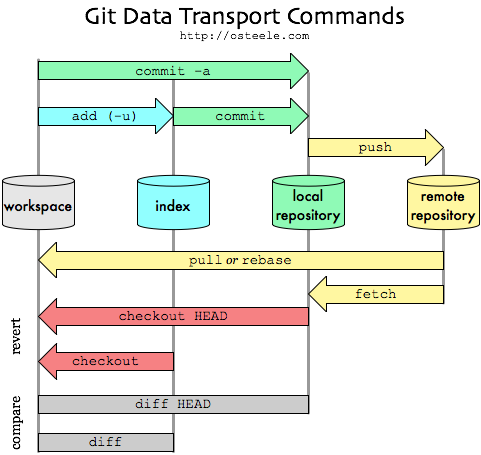
\includegraphics[scale=0.7]{pics/git-transport} \\

   \end{itemize}

\subsubsection{GitHub or gitlab}
\begin{itemize}
\item For gitHub, I have two github account:
\begin{enumerate}
  \item zhaoyan.hrb@gmail.com  zhaoyan;
  \item yan.zhao.74@gmail.com YanZhao
\end{enumerate}
A project hello-world, Main project is on zhaoyan, then I use YanZhao account fork main project. project link is : \\
git://github.com/zhaoyan/hello-world.git(read only) \\
git@github.com:zhaoyan/hello-world.git(modifiable)


\item \linuxcommand{ssh-keygen -t rsa -C yan.zhao.74@gmail.com} \\
    \item your public key has been saved in /c/Users/zhao/.ssh/id\_rsa.pub(for windows) ~/.ssh/(for Linux). Then you should paste the public key to the account in github.com.  
        	
   \item You can copy id\_rsa.pub and id\_rsa to other computers. so you don't need to run ssh-keygen command any more. But when you copy id\_rsa to linux or Mac, you need \linuxcommand{chmod g-r id\_rsa} to make your private key only readable for you. Or when you push or fetch, git will refuse your request.  (ssh -v will give you verbose information. you must restart ubuntu after you move id\_rsa to ~/.ssh).


    \item once you finish it, \linuxcommand{ssh -T git@github.com} will test you key setting. (github has details explanation.)

\item In your .ssh directory, you find a id\_rsa command, don't change it. You can build or modifiy config file in ~/.ssh diectory. Add something below. 1) you can use your own id\_rsa\_old name here, how to use ssh-keygen to product different name, you can see manual. 2) \textbf{Don't add Port 443 statment first, if you use ssh -T to get no response, then add Port 443, then it will work}.
		\begin{verbatim}
		Host github.com
		   Hostname ssh.github.com
		   Port 443
		   IdentityFile ~/.ssh/id_rsa_old
		\end{verbatim}

    \item Sometimes, you can't see project link, you can click the little eye(watchers) on the right upper corner. pull request will show up.

\item \textbf{Don't use any Chinese in version control, If your English is not good, use
    Pinyin.}
    
\item In order to do anything in Git, you have to have a Git repository. This is where Git
    stores the data for the snapshots you are saving. There are two main ways to get a
    Git repository. \textbf{One way} is to simply initialize a new one from an existing
    directory, such as a new project or a project new to source control. \textbf{The
    second way} is to clone one from a public Git repository, as you would do if you
    wanted a copy or wanted to work with someone on a project.
\end{itemize}

\subsubsection{GUI}
\begin{itemize}
	\item There are two main GUI usages in git: 1) gitk 2) gui diff and merge    
    \item gitk is GUI application. gitk --all will list all the branches.
    \item For gui diff and merge.  You need to download diff and merge application first. For Linux, meld is the best option. You need to change you .gitconfig to add [diff] and [difftool] section. Pay attention. They finish the same task. Make you \linuxcommand{gui difftool} invoke the GUI diff(merge) application.  
       
      \item For Mac, I haven't test if meld can be used. But I have tried diffMerge, On its website, you can find how to config .gitconfig file.
      \item For diff, you will not change git diff command. Only git difftool invoke GUI. For Merge, git merge just modify your file in work space to diff format when there is conflict. Then you need to run \linuxcommand{git mergetool} to invoke GUI application.  Just remember: \textbf{First run git merge, if conflict, then git mergetool}
      \item When you use meld in Linux, just add below into .gitconfig 
\begin{verbatim}
[merge]
    tool = meld
\end{verbatim}
\item When you run \linuxcommand{git mergetool} Meld will open three panel windows. Middle one is your result. left and right are two conflict branches.  When you finished. just click save and exit. Then run \linuxcommand{git status}, you can see it is ready for to add and commit. 
 
\item For other mergetool, you maybe need more complex configuration. Detail can be found on mergetool website. 
\begin{verbatim}
[merge]
tool = kdiff3
[mergetool "meld"]    % or "P4Merge" in Windows
path = /usr/bin/meld
keepBackup = false
trustExitCode = false	
[diff]
tool = p4merge
[difftool "p4merge"]
path = C:/Program Files/Perforce/p4merge.exe
\end{verbatim}
\end{itemize}

\subsection{Basic commands}
\subsubsection{status log show}
\begin{itemize}
		\item \linuxcommand{git status}  you need to use this command very often. 
		\item  \linuxcommand{git status -uno} will not show untracked files. \linuxcommand{git log --author=Bob} only show Bob's commit.

		\item \linuxcommand{git status -s} show two columns , the first is staging, the second is working tree. if you modify a file,  then add. then you modify a file again. Now git status -s show MM a. guess what it means. 
	\item \linuxcommand{git log} can show you all the commits history. 

\begin{verbatim}
git log --pretty=oneline #just show simply log information
git log -p   #show ci log and source modification each commit.
git log -2  #just last two commits
git log --after 2015-12-01  #show all commits after date
git log --oneline  #simple informaitons
git log --abbrev-commit --pretty=oneline #simple informaitons
git log experiment..master #show commits on master, not on experiment
        a--b--e--f(master)
            \c--d(experiment)
git log origin/master..HEAD #what have you push to remote?
\end{verbatim}

   \item \linuxcommand{git show} to examine a single object. such as \linuxcommand{git show v1.0} and\linuxcommand{git show master:book.tex} will output source file.  It can used on commit(just like log command), or tree (just like cat-file -p). or plain blobs,(just like cat-file -p). 
 \end{itemize}

\subsubsection{add commit}
\begin{itemize}

		\item When you add  a file, a blob object is produced, and .git/index(binary file) is updated to include it. You can use \linuxcommand{git status -uno} to hide all untraced files. You also can produce a .gitignore file in you project, it will work on present and all children directory. When you use \linuxcommand{git status}, It will not show so many untracked files.  Example is below. edit .gitignore file.
\begin{verbatim}
# comment
*.a   #ignore all files with .a extention
!lib.a  #but include lib.a
build/   #ignore all file in build directory
doc/*.txt  #ignore all txt files in doc/ but doc/server/arch.txt will be included.
\end{verbatim}

\item You should avoid using \linuxcommand{git add .} to add so many unnecessary files. If you run it accidentally,  You can use \linuxcommand{git reset} to revert add which you just ran. 

\item When There are a lot of files to add, \linuxcommand{add -i } is a good choice.  \linuxcommand{add -u} will only add tracked files, no dot is needed. 

\item Current working directory is (1),   Index file or staging is (2) and  Git local repository is (3) \\
      (1) -> (2) -> (3) \\
  \linuxcommand{git add} (1) -> (2) \\
   \linuxcommand{git commit} (2) -> (3) \\
   \linuxcommand{git commit -a}  (1)->(3) Don't recommend use it. \\

    \linuxcommand{git add .}   add all files. Be careful to use this command   \\
    \linuxcommand{git add -u}   it's very often used command. or It can be used in such senorita: rm *.txt, then git add -u will delete *.txt from staging. \\
    
    \item commit command usually don't pay attention to files or directory, it just product a commit to produce a sha object(commit). 

   \item \linuxcommand{git commit --amend}  don't produce new commit, just modify last commit.
   
   \item If you add a file a.c, but you don't commit it. How to revert? \linuxcommand{git reset a.c} Will remove a file named a.c from the current index, the "about to be committed" area, without changing anything else.  contrary to  \linuxcommand{git add --a.c} To undo git add . use git reset (no dot).
   
   \item If you haven't commit yet, so you can't use reset now. At this time you can use \linuxcommand{git rm} command. 
   
   \item If you add a file a.c, and you commit. How to revert? use \linuxcommand{git rm} or \linuxcommand{git rm --ached}, then commit it again. 
   
   \item Previous method will produce two commits. if you want to just modify current commit.  git rm first, then use \linuxcommand{git commit --amend}.  Or you can also use \linuxcommand{git reset HEAD~}, then maybe you need git add or not, depends on your context. last \linuxcommand{git commit -c ORIG\_HEAD}.  Here reusing the old commit message. reset copied the old head to .git/ORIG\_HEAD; commit with -c ORIG\_HEAD will open an editor, which initially contains the log message from the old commit and allows you to edit it. If you do not need to edit the message, you could use the -C option.     

   \item Both(commit --amend) and (reset... commit again) will produce new commit. In fact, any commit sha include current operation second. So it will different. 
   
   \item \textbf{So don't change commit which you pull from public or you have pushed to public} 
        
   \item \linuxcommand{git ls-files --stage} will show all the files in stage(index).    
\end{itemize}

\subsubsection{remove rename}
\begin{verbatim}
git rm a // It will delete from work space and index
git rm --ached a  //just delete a from index.
git commit -m "delete file a"

git mv a b  #is three command: mv a b; git rm a ; git add b ;
git commit -m "rename a to b"
\end{verbatim}

\subsubsection{diff}
\begin{itemize}
\item diff basic usage. 

\begin{verbatim}
git diff     ##(1) and (2)
git diff -cached   ##(2) and (3)
git diff HEAD   ##(1) and (3)

git diff tag     ##tag and HEAD
git diff tag file    ##just compare a file (only one file name)
git diff tag1..tag2   ##two tags( you can omit two dots)
git diff SHA11..SHA12  ## two commits
git diff tag1 tag2 file or  git diff tag1:file tag2:file

#tag can be a alias of remote
git remote add xjsff git://github.com/xjsff/hello-world.git
git diff xjsff/master README  ##local README and README in xjsff/master
\end{verbatim}
		\item \linuxcommand{git diff --name-only} just show changed files name. so you can compare it one by one.  \linuxcommand{git diff --name-status} will show how do you changed files, add, delete or modify. 

		\item Before checkout or reset, you'd better to use diff command to see if there are important content to avoid overwrite. that is a good habit. 

		\item    diff -u is good command, it will show context of difference.  All the differences give by differences section.
   
\item  After git fetch, you can use \linuxcommand{git diff master origin/master} to see all the modifications, then decide if you want to merge. fetch+merge is better than pull.
   
\item \linuxcommand{git difftool -- file} to use meld to see the difference, it looks much better.
\end{itemize}
\subsubsection{checkout reset}

\begin{itemize}
		\item \textbf{branch->commit, HEAD->branch, When not follow paths, checkout move HEAD, reset move (HEAD->branch, HEAD must point to a branch). } It's helpful for you to understand these two command.
		
		\item If HEAD->master, reset will move HEAD->master together, if HEAD->commit, reset will only move HEAD. at this time, It's still detached head status. 
		
		\item There are two basic different usages for checkout: 
		\begin{enumerate}
		\item with paths(file), it just with <commit> to replace index and work space. At the same time, It will not change HEAD. 
		\item without paths, if you follow a branch it will move HEAD to branch.
		\item without paths, if you follow a old <commit>, It will move HEAD to old <commit>. HEAD will be a ref to a branch,  When It points a real old commit, It will be "detached HEAD" and all commits after HEAD may be discards in the future. 
		\item \linuxcommand{checkout commit <commit> -- paths} or \linuxcommand{checkout branch}. Don't use in\linuxcommand{git checkout <commit> (empty)} without paths, It will put HEAD in detached state. \textbf{After checkout, follow a branch, or follow /patth/file name.}
		\item \linuxcommand{git checkout} just like \linuxcommand{git status}
		\end{enumerate}
				
		\item When checkout and reset follow file, they can be a file, *.cpp(some files) , . (all files),  /path\_name(path\_name and recursive) and /path\_name/*(no recursive). 

	 \item If you are in detached HEAD state, 1)You don't modify work space, just use checkout master to set HEAD to master again. 2)If you modify work space and you want to keep it. commit it first, remember <commit-sha>. Then checkout master. merge <commit-sha>. Then HEAD will move to master and master will point to merged commit.  
	 
\item If without commit, only file, it will use file in index to overwrite work sapce. \linuxcommand{git checkout . or git checkout file} (2)->(1). 

\item If there is commit, \linuxcommand{git checkout HEAD .}  (3)->(1) and (2) dot represents all the files. \textbf{This is a dangerous command. Save or commit you local work first.}
    
\item checkout will overwrite work space directly, it is not like merge, and doesn't produce conflict files. So be careful!

 
\item you can checkout a file from different history. :
\begin{enumerate}
\item \linuxcommand{git checkout v1.2.3 -- filename}  tag v1.2.3 

\item \linuxcommand{git checkout stable -- filename}  stable branch 

\item \linuxcommand{git checkout origin/master -- filename}  upstream master 

\item \linuxcommand{git checkout HEAD -- filename}   the version from the most recent commit 

\item \linuxcommand{git checkout HEAD\^{ } -- filename}   the version before the most recent commit 

\item \linuxcommand{git checkout xxxx  --filename} xxxx is commit version number.
\end{enumerate}


\item  Similarly, There are two different usages for reset: 
\begin{enumerate}
\item with paths, it will not move HEAD and master (reset commit). \linuxcommand{git reset <commit>-- <paths or filename>} will overwrite index with commit, (3)->(2).  it just like contrary operation of add.

\item Without paths, it will reset (HEAD-->master) together to a new <commit>, and all commits after reset commit will be discards( delete commits, dangerous!). Because It reset (HEAD-->master) together, then It doesn't have detached head problem.  

\item Without paths, there are three options you can use:
\begin{verbatim}
git reset [--soft|hard|mixed ] <commit>
## soft just reset commit
## mixed reset commit and (3)-->(2)
## hard reset commit and (3)-->(2)-->(1)
\end{verbatim}
\end{enumerate}

\item How to save from wrong reset command? When you reset to a <old-commit>. All the commits after <old-commit> will not found easily unless you can remember all the commit sha value.  A better method can be use \linuxcommand{git reflog show master | head -5}. It will show master@{0...n}. It represent all the master ref history. You also can use it to show head moving history.      

\item HEAD@{num} can be used as follow to change commit history after a <old-commit>
\begin{enumerate}
\item \linuxcommand{git checkout <old-commit>} \# detached head
\item \linuxcommand{git commit ...} \#last commit sha is 123abc
\item \linuxcommand{git checkout master} \# move head to branch
\item \linuxcommand{git reset --hard HEAD@{1}} \# reset it to old commit 123abc.  
\end{enumerate}

\item followed by <old-commit>, both checkout and reset --hard will modify all files in work space. 

\item If you modify a file in (1), you can restore it from (2) with \linuxcommand{git checkout --a.c} or from(3) with \linuxcommand{git reset HEAD --a.c}.  They will overwrite (1) forever, so be careful. If you want to keep it, you can do:
\begin{verbatim}
git add filename  ##save modify to (2)
git checkout v1.2.3 filename  ##get old version
git diff   ## compare
git checkout filename  ##restore
\end{verbatim}
\end{itemize}

\subsubsection{stash}
\begin{itemize}
		\item Sometimes I have a situation that I am working on some feature on my own branch and suddenly someone comes to me and says that something really important has to be fixed or improved on the main branch. Usually it happens when I am in the middle of very important changes which are not ready to be committed for some reason. 

\item Normally, I would have to save the changes (diff) into some file, switch to the main branch abandoning any changes, apply the fix or improvement and commit it. Then I could switch back to my own branch, apply the changes (patch) from the file and continue the work. While it is not something difficult, it can be done much easier with Git.

\item When you use \linuxcommand{git stash}, It will run \linuxcommand{git reset --hard} automatically. so all you work will disappear. you can use \linuxcommand{git statsh pop }to revert it.

\begin{verbatim}
You need to modify a bug in release version. First stash, then checkout release. coding....,commit,last git stash pop.
git stash save "you messaage" #
git stash list #list all stash
git statsh pop #
\end{verbatim}

\end{itemize}

\subsubsection{rebase revert}
\begin{itemize}

\item Reverting has two important advantages over resetting. First, it doesn't change the project history, which makes it a "safe" operation for commits that have already been published to a shared repository. For details about why altering shared history is dangerous, please see the git reset page.

\item Second, Git revert is able to target an individual commit at an arbitrary point in the history, whereas git reset can only work backwards from the current commit. For example, if you wanted to undo an old commit with git reset, you would have to remove all of the commits that occurred after the target commit, remove it, then re-commit all of the subsequent commits. Needless to say, this is not an elegant undo solution.

\item revert will produce a new commit too. \verb=git revert HEAD^^ = produce a new commit

\textbf{Never rebase branches or trees that you pulled. Only rebase local branches.
Never ever rebase a branch that you pushed, or that you pulled from another person}
\par rebase will change history, if you don't have valid reason to use it, just use merge
command.

\item rebase command and merge command is little different. \textbf{When you are in test branch, master branch has a new commit, You can rebase on new commit on master. Because in the end, your test branch will be merged back to master, rebase often can save you a lot of conflict problem in the future. }

\item \textbf{When you in the master branch, and When test branch has finished or partly finished, You can use git merge command to merge test branch into master branch}

\item You can think merge and rebase are two commands operate on branch.

\item rebase basic usage.
1) in master  branch , commit a new commit (m1), in test branch, commit few times(t1..t2). \\
\begin{verbatim}
   t1-->t2
 /
m-->m1
\end{verbatim}
2) checkout test branch, then \linuxcommand{git rebase master.} /* means that SHA value has been changed.\\
\begin{verbatim}
       t1*-->t2*
      /
m-->m1
\end{verbatim}

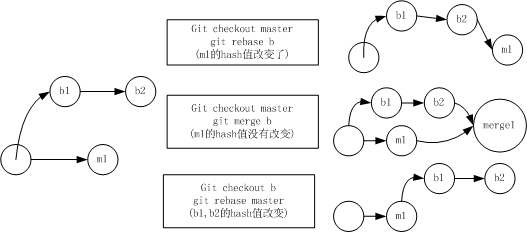
\includegraphics[scale=0.7]{pics/Git_rebase} \\

\item rebase has --onto options. Detail can be found in git rebase document. Just google it. 

%rebase的命令和merge的命令有点不太一样。一个标准的流程应该是从master创造出一个分支test,然后在test commit 几次。
%同时在master commit 几次。这个时候,进入master分支,git rebase test,

%1)如果b是一个本地的branch,如果master上没有m1那么在master 上,执行 git rebase b 和git merge b效果一样,就是增加两个新的commit。 \\

%2)如果master 上也有个更新m1。那么需要注意,如果m1只是本地的(你不是pull,同时,你还没有push)同时,你还希望保存
%b1 和 b2 两次commit。这个时候,可以使用git rebase b. (因为m1 hash值改变了,所以必须要保证本地化)。\\
%3)如果master上m1不是本地化的,那么你最好用merge。但是当你删掉b分支以后,b1,b2消失了。\\

%4)如果master上m1不是本地化的,你也可以进入b分支, 然后git rebase master,(不过你需要注意,这个时候,你还在b分支里面。)然后git checkout master , git merge b。
%相当于把b当中的b1和b2,放到了m1前面,(m1的hash没变,相当于增加了两个新的commit b1和b2. 你还需要保证b是个本地的branch)
%一句话:rebase的使用需要谨慎使用,他的本意是修改历史的作用,如果你没有很明显的理由,就直接用merge好了。\\

%rebase branch1 有三个含义,1)当前不在branch1中,2)branch1为焊接接入点,3)当前的分支commit的值改变了。

%rebase branch 与rebase master是有区别的。如果你当前在master中,并且以master为主线,那么就应该调用rebase branch。从这个角度上来说,rebase master应该用的不多。除非是上面说的第4种情况,那就是m1已经push出去,并且别人也在用。

%rebase两种常用场景,第一就是本地的分支上,两个分支出现并行情况,通过rebase branch1,可以得到相对干净的历史commit. 第二就是rebase thorn/master, 把别人的工作集成到我的master中去,(thorn/master和master都发生了commit)生成一个更干净的历史。他的基本原理和merge大致相同。

\end{itemize}

\subsubsection{branch merge}

\begin{verbatim}
git branch -r  # list all the branches on the remote
git branch #list all the local branches
git branch -D b1 #delete the b1 branch
git checkout branch-name # switch to branch-name
git checkout -b new-branch master # build new new-branch from master and switch to it.
git checkout -b newbranch # build newbranch
git checkout -b newbranch origin build newbranch based on origin
git branch -m master mymaster # rename the branch
git push origin branch ,//this command will push branch to github. \\
but push branch to server isn't very meaningful, at least I think so. \\
\end{verbatim}

\begin{itemize}
  \item merge command is followed by two branches, no files name.  such as \linuxcommand{git merge
      origin/master master}

  \item merge will produce a new commit without conflict,  If there is a conflict, you need manually resolve it, then commit it manually.

      \item When merge can't resolve conflict, it will put working tree into a specify conditions. (file in work space has been modified with conflicted format)
      
   \item Three kinds of merge. 1) straight merge. 2) squash merge, 3) cherry-pick
\item \linuxcommand{git merge-base b1 b2}  found the common ancestor
\item \linuxcommand{git cherry -v master test}  in master branch, found all commits in test, but not in master.
%在master分支中,找到所有test中有但是master中没有的commit.

%主要用于将两个或两个以上的开发分支进行合并。
%主要有三种merge.第一种为straight merge. 他把一个分支的整个历史合并到另外一个分支当中去。
%还有一种就是squash 把所有的历史变成一个历史commit。 git merge --squash contact。针对于squash,
%你需要merge以后再提交。最后一种就是cherry-pick,
%git chekcout master git cherry-pick 321d76f (这是在另外一个分支提交的)。
%当然1你也可以git cherry-pick -n 321d76f. -n 告诉git先不提交,然后你就可以继续cherry-pick了。
 %然后 git commit 不用-m,这个时候一个默认的编辑器就打开了。
 %所有你pick的commit message就会自动出现在那个编辑器中。

%当merge命令自身无法解决冲突的时候,它会将工作树置于一种特殊的状态,并且给用户提供冲突信息,
%以期用户可以自己解决这些问题。当然在这个时候,未发生冲突的代码已经被git merge登记在了index file里了。
%如果你这个时候使用git diff,显示出来的只是发生冲突的代码信息。

%在你解决了冲突之前,发生冲突的文件会一直在index file中被标记出来。这个时候,如果你使用git commit提交的话,
%git会提示:filename.txt needs merge 在发生冲突的时候,如果你使用git status命令,那么会显示出发生冲突的具体信息。\\

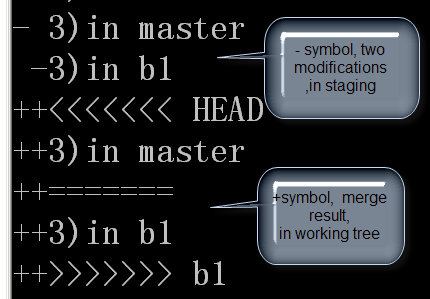
\includegraphics[scale=0.6]{pics/merge-diff} \\

after you resolve conflict 1) git add filename 2) git commit


\item If you want to revoke a branch to a status before merge 
%如果你希望撤销一个分支到merge前的状态,那么使用如下命令:\\
git reset --hard HEAD --hard means working tree and index file both restore.
Or, if you've already committed the merge that you want to throw away, use this command: \linuxcommand{git reset --hard ORIG\_HEAD}.

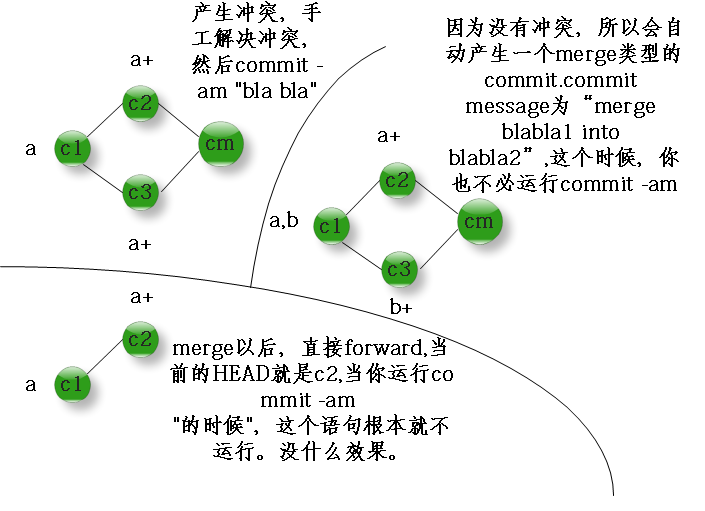
\includegraphics[scale=0.5]{pics/git-merge} \\
\end{itemize}

\subsubsection{remote push pull}
\begin{itemize}

\item don't use pull, just use fetch, then merge. 
When you run \linuxcommand{git merge origin/master master}, there are three possibilities. \\
1) Working directory no modification, then fast-ward merge and working and index will be updated. \\
2) Working directory has modification, merge will fail. \\
3) Working directory has modification and commit, merge maybe ok, then working and index will be updated. merge maybe conflict, then use merge tool to resolve conflict and commit to produce a commit manually. \\

\item origin is a alias of remote repository,  \linuxcommand{git remote add origin
    git@github.com:zhaoyan/test.git}just give a alias name, It will not real create remote repository, you need to log in github to create it manually.  Beside add, you can show, rename and delete a these alias. with these alias, you can \linuxcommand{push or fetch origion} directory, don't need to write the address of the remote repository.

\begin{verbatim}
git remote add paul git://github.com/paul/test.git
git remote -v
git remote show paul #show paul all the informations, including branch.
git remote rename paul pa
git remote rm pa #delete pa, because he will not contribute the system.
\end{verbatim}

\item push command is followed by a repository name and a branch name.  such as \linuxcommand{push origin master}. It has a lot of syntax, can be use change remote branch name and delete remote branch.
\begin{enumerate}
\item git push origin experiment \#push a branch to server
\item git push origin local:experiment \#change local branch name, and push to server.  \item git push origin :experiment \#delete local branch ,use empty name 
\item git push origin erperimental:experimental-by-yan \#give remote-tracking-branches other name,here experimental-by-yan is remote-tracking-branches name,erperimentallocal name. <source-name>:<destination-name>
\end{enumerate}

\item When you push a local branch to remote, sometime it will produce non-fast-forward error. Reason is
    demonstrated by below two figures:
\begin{verbatim}
       (master)
           |
C1-->C2->C3(origin/master)
\end{verbatim}

\begin{verbatim}
             C4 (master)
           /
C1-->C2->C3(origin/master)
\end{verbatim}
\item In one word, from master, you can't reach origion/master, (each commit only has parent pointer).  In order to
push successfully, you have to \linuxcommand{git fetch origin} and \linuxcommand{git merge origon/master
master} firstly. Then automatically produce a new commit or manually resolve conflict and commit manually. it
will produce:
\begin{verbatim}
             C4-->C5 (master,  origin/master)
           /         /
C1-->C2->C3
\end{verbatim}


\item If commit history look like below, you can push it successfully.
\begin{verbatim}
 (origin/master)
           |
C1-->C2->C3(master)
\end{verbatim}
\end{itemize}
\subsubsection{blame} 
    \begin{verbatim}
    git blame -L l2,l3 hello.html
    \\Who made some modification.
    \end{verbatim}


\subsection{Branch}
\begin{itemize}

\item Branch can be in  two different positions. One is in the local place, you can use git branch to check them. The other is remote-tracking branches, you can use git branch -r to check them. They have origin/remote-branch-name, origin is not branch name, it's repository  name. 

\item Usually, there are three common use branches. One is release branch which can be based on one release commit. Usually, it used to fix some bugs in release, then you can merge back master branch. Another is feature branch, when you add a feature, and you don't know if it's good or can be finished properly, you can produce a feature branch. The last branch is vendor branch. You don't commit on it. just keep track with upstream new version , then merge back with you master branch.

\item You can't checkout remote branch, such as \linuxcommand{git checkout origin/branch1}. In order to do so , you have to create a local branch based on remote branch, such as \linuxcommand{git checkout --track -b branch1 origion/branch1}, then work on the local branch1. after you finish it, you can push it back. with --track, you can push or fetch without specify remote repository name. you can omit it.

\item when you want to emerge mother's work, you'd better build a branch first.

\item Branch is based on commit,  When you merge a branch back to  master, you may delete it if you don't need it anymore.

\end{itemize}

\subsubsection{branch daily usage }
\begin{itemize}
\item single person, center control, with branch. 	when you finish the branch, you can merge it with master. 

\item Below figure show two different position are working on the same branch--malouf. \\

	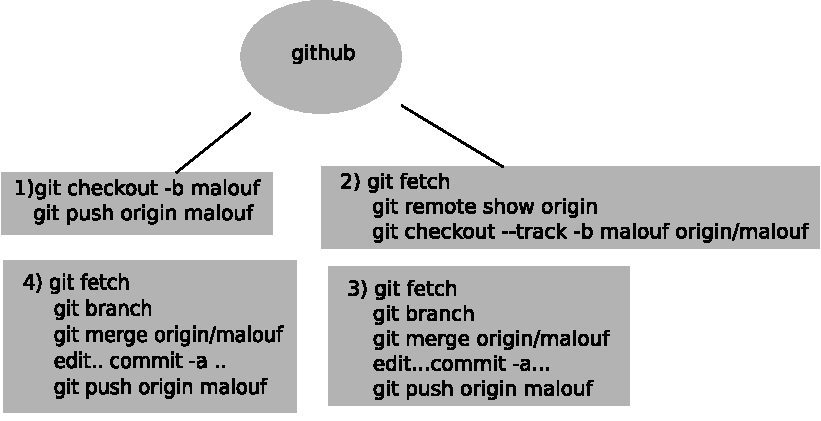
\includegraphics[scale=0.6]{pics/git_branch} \\
   
\item Multi person, center control, with branch 

   \begin{enumerate}
     \item \linuxcommand{git fetch upstream} get zhaoyan upstream the updated development process.
     \item \linuxcommand{git checkout -b test\_bla upstream/master} based zhaoyan master branch, build local branch test\_bla (any name is OK.)
     \item edit,  compile, \\
     git commit -am "s1" \\
     edit,  compile,  \\
     git commit -am "s2"\\
     While, upstream/master maybe changed,  a new commit t1 appear.
\begin{verbatim}
     s1--- s2
____/___t1
\end{verbatim}
\item \linuxcommand{git fetch upstream} when you want to update upstream, you have to get new commits

\item \linuxcommand{git merge upstream/master} If no conflict, produce a forward merge, if conflict, manually
    resolve and commit a new commit. \linuxcommand{git commit -am "st1"}
\begin{verbatim}
      s1--- s2
____/___t1___\st1__
\end{verbatim}

\item Or, you can use the second method: \linuxcommand{git rebase upstream/master} No conflict, produce a new commit. with conflict, manually resolve it, then \linuxcommand{git add conflict\_file}, then
    \linuxcommand{git rebase --continue}, not need to commit.
    \begin{verbatim}
        t1---s1*--- s2*
____/
\end{verbatim}

\item git push origin test\_bla

\item login github, look for you repository, checkout test\_bla, then click "request pull" button.

\item If other accept you request, you can delete test\_bla branch. \linuxcommand{git branch -D test\_bla}

\item \linuxcommand{git push origin  :test\_bla}  delete test\_bla branch in github.
\item  repeate 1-10.
   \end{enumerate}
\end{itemize}

\subsection{History}
\subsubsection{history representation}
\begin{itemize}
\item No space in tag name.
\item Common used history commit ref name. 
\begin{verbatim}
FETCH_HEAD,ORIG_HEAD, COMMIT_EDITMSG:
HEAD:  #last commit
MERGE_HEAD:
FETCH_HEAD:

HEAD^: HEAD's parent, it's ORIG_HEAD
HEAD^ or HEAD^1   # first parent
HEAD^^ or HEAD^2 # second parent
HEAD~4 : HEAD

HEAD:README.txt
%It represents a blob object,sh-hash value of blob is not easy to see.
\end{verbatim}

\end{itemize}

\subsubsection{history change}
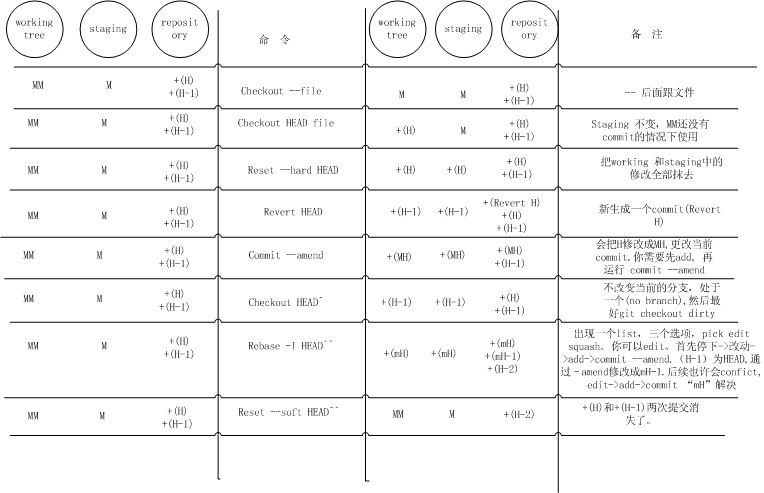
\includegraphics[scale=0.6]{pics/Git-history} \\
\begin{itemize}
\item \textbf{Three basic modification history usage:}
\begin{enumerate}
\item Delete or combine certain commits;
\item Delete new commits after a point
\item Delete old commits before a point
\end{enumerate}

\item \textbf{Three common commands for modification history: checkout, cherry-pick and reset. Other useful command is rebase, you can think that it's a combination of previous three commands. }


  \item \textbf{Change current latest commit} \linuxcommand{git commit  --amend} not only change the message, but
      also the working tree contents. \linuxcommand{git commit -C HEAD\^{}}
        will produce a new commit, but this commit is just like \verb=HEAD^ =.

  \item \textbf{Delete some new commits} \linuxcommand{git reset --hard  HEAD\^{}\^{}\^{}} will delete \verb=HEAD^^=  and \verb=HEAD^=  and HEAD three commits forever, It's is a dangerous command, be careful about it.
   
\item \textbf{Delete all old commits before A} \\
1)\linuxcommand{echo "Commit from tree of tag A | git commit-tree A\^{}\{tree\}}  It will produce a <SHA value>. This command will produce a new commit with <SHA value> and without any parent. It's a root commit. 
2)\linuxcommand{git rebase --onto <SHA value> A master}  All the history behind of A will be deleted. \\

  \item \textbf{Delete some old  commits by cherry-pick } \\
   1)\linuxcommand{git checkout C}, C is a tag, by now, working tree
      is C status, Here, you can't use
      \linuxcommand{reset C}, because it will put master to C,  then D, E and F will become a unreferenced
      commit, deleted by Git. If no D,E and F,
You can't use cherry-pick in the next steps.     \\
2) \linuxcommand{git cherry-pick E and F} , delete D commit ,cherry pick will produce a new commit SHA value. just like rebase.\\
3) \linuxcommand{git checkout master }  It will end Head detached status.  \\
4) \linuxcommand{git reset --hard HEAD@\{1\}}. reset HEAD-->master to new F* commit. 


  \item \textbf{Delete some old commits by rebase } \\
  1a) \linuxcommand{git rebase --onto m2 m3 m5}, You need to know that  m3 m5 will not m3, It will produce a new commit m4 and m5,
   SHA value will be different. And from the figure, you can see that master branch is still on old m5 commit.  so you need perform step 2. \\

%\begin{figure}
%  \centering
%  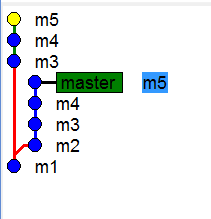
\includegraphics[scale=1.0]{pics/rebase1}
%\end{figure}


  1b )\linuxcommand{git rebase --onto m2 m3 master} will keep you track master branch, after that you don't
  need to run step 2 below. It will be easy way to do that. \\

  2) \linuxcommand{git checkout master }  and \linuxcommand{git reset --hard HEAD@\{1\}}. After these two commands, you can see m2 has disappeared. \\
%\begin{figure}
%  \centering
%  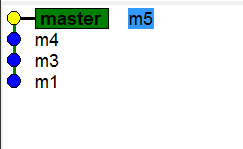
\includegraphics[scale=1.0]{pics/rebase2}
%\end{figure}

  \item \textbf{Combine two old commits by cherry-pick} \\
  1)\linuxcommand{git checkout D}, D is a tag, by now, working tree is D status,  \\
  2) \linuxcommand{git reset --soft B } ,  because HEAD is D now, go to B, --soft means working tree is still D status \\
  3)\linuxcommand{git commit -C C }  then \linuxcommand{git cherry-pick E and F}. \\
  4)\linuxcommand{git checkout master }  \linuxcommand{git reset --hard HEAD@\{1\}}. Detail can be found in "Got Git". \\

\item \textbf{Combine two old commits by rebase} \\
  1)\linuxcommand{git checkout D}, D is a tag, by now, working tree is D status,  \\
  2) \linuxcommand{git reset --soft B } ,  because HEAD is D now, go to B, --soft means working tree is still D status \\
  3)\linuxcommand{git commit -C C }  \\
  4)\linuxcommand{git tag newbase} \textbf{give a tag name to avoid remember sha-value} \\
5)\linuxcommand{git rebase --onto newbase D master}  then check \linuxcommand{git branch }to see if it's on branch master, if it's yes \\
6) \linuxcommand{git tag -d newbase } \\  Detail can be found in "Got Git". \\

\item \textbf{difference cherry pick and rebase} \\
1)rebase and cherry pick will change commit SHA value, so don't use
    it on any commit that you have pulled or you have
    pushed. cherry pick will not change \\
2)cherry pick should be used in change few commits, and rebase can be used to change a lot of commits at the same time.  \\


\item \textbf{delete all the commits in a merged branch}

\begin{figure}
  \centering
  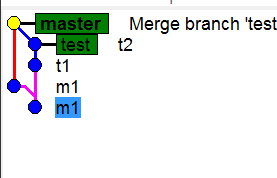
\includegraphics[scale=1.0]{pics/rebase3}
\end{figure}


1) \linuxcommand{git rebase -i -p  --keep-empty --onto 9f843b 9f843b master} -p means keep merge commit.
9f843b is m1 commit. \\

2)In git-rebase-todo file, you can see all the commits. for merge commit, you need to change it to
\linuxcommand{x git cherry-pick --allow-empty -m 1 <SHA>}, comment all the unnecessary commits. Then you
can see close this file. and rebase -i will run it according to this file. \\

3) Maybe you need to run \linuxcommand{git checkout master }  \linuxcommand{git reset --hard HEAD@\{1\}}
and \linuxcommand{git branch -D test} to make history clean.  (x options in msysGit system doesn't work, you
need to manually git cherry-pick, any way, you can see all the SHA with gitk --all command. )

\end{itemize}


\subsection{Daily usage}
\subsubsection{clone a project from github}
\begin{enumerate}
\item  \linuxcommand{git clone git@github.com:zhaoyan/hello-worl.git}  you can copy the address from github
    website. I think that it will produce origin alias automatically.
\item modify... main.cpp
\item \linuxcommand{ git add main.cpp}  \linuxcommand{git commit  -m "modify sth..."}
\item \linuxcommand{ git log} to see if you have commit successfully.
\item \linuxcommand{git remote -v } to see what origin is.
\item \linuxcommand{git push origin master }   This command works only if you cloned from a server to which you have write access and if nobody has pushed in the meantime. If you and someone else clone at the
    same time and they push upstream and then you push upstream, your push will rightly be rejected. You'll
    have to pull down their work first and incorporate it into yours before you'll be allowed to push. (detail can be
    seen in the previous push command: produce non-fast-forwarderror.
\end{enumerate}

\subsubsection{Add a project to a git}
\begin{enumerate}
  \item \linuxcommand{cd test}, run \linuxcommand{git init}
  \item \linuxcommand{touch test.cpp}, then \linuxcommand{git add test.cpp} or \linuxcommand{git add .} dot
      means all the files. Directories are added automatically when adding files inside them. That is, directories
      never have to be added to the repository, and are not tracked on their own. You can say "git add <dir>" and
 it will add all files in there.
  \item \linuxcommand{git rm README}  you can delete a file
  \item \linuxcommand{git commit -m "first commit" } or \linuxcommand{git commit -a -m "first commit"} This is
      simple form. Combine add and commit together. Git commit -a can't add new files. If you add some news
      files, you should use \linuxcommand{git add newfile}. then commit.

\item \linuxcommand{git log} or \linuxcommand{git status} After committing, you can use log command to
    check if it has been submitted successfully.

\item    \textbf{then, login github, create repository with name test}

\item \linuxcommand{git remote add origin git@github.com:YanZhao/test.git}
		
\item 		\linuxcommand{git remote -v }you can check remote repository
\item 		\linuxcommand{git push -u origin master} 	You can not emit origin, if you don't specify branch, default
    is master. master is default local branch, you don't need to create it explicitly. this command push local
    content
to the server.
\end{enumerate}


\subsubsection{update a project from github}
\begin{enumerate}
\item  \linuxcommand{git clone git@github.com:zhaoyan/hello-worl.git}  you can copy
    the address from github website.
\item modify... main.cpp
\item \linuxcommand{ git add main.cpp}  \linuxcommand{git commit  -m "modify sth..."}
\item \linuxcommand{git log} to see if you have commit successfully.

\item \linuxcommand{git fetch}  to get origin/master.

 \item \linuxcommand{git diff master origin/master} maybe you need to resolve conflict before you push.
\item \linuxcommand{git merge origin/master} If there are difference, you need to merge before you push, or it
    will produce non-fast-forward error.  default is local master branch, you can't write in "git merge master" to
    skip "origin/master".
\item \linuxcommand{git push origin master}

\end{enumerate}

\subsubsection{Collaborate With Applications}

\begin{itemize}
  \item For codeblock, project file is pro1.cbp, It will produce two directory bin and obj, you need to modify
      .gitignore file, add bin/ and obj/ to ignore. good suggestion.
  \item For kdevelop:
 \begin{enumerate}
\item rm Makefile.in or .svn (if there are) 
\item go into the src directory, and run git init 
\item git add . and  git commit 
\item git remote add origin git@github 
\item git push origin master 

\item another kdevelop, rm src
\item git clone git@github src
\item modify Makefile.am with you kdevelop project file.
\item in configure dialog, Configure options->linker flager -> add -L./ and add lib to the debug/src directory.
\item compile and run.
\end{enumerate}  


  \item For latex,  Only *.tex *.bib( reference)  and /pic directory are useful, You need to add them
      manually.
\end{itemize}

\subsubsection{single person on different computers }
On computer 1:
\begin{enumerate}
    \item \linuxcommand{git log HEAD..origin}  to check if there are differences. if true
    \item \linuxcommand{git fetch,  git merge origin/master master} ( git fetch give you more chance to
        examining it, it's better than pull)
    \item \linuxcommand{git commit -a -m " "}
    \item \linuxcommand{git push}
    \item  \linuxcommand{git log HEAD..origin }check push successfully
\end{enumerate}

On Computer 2: \\

Same operation, when you merge, it will only produce forward merge, it's relatively easy.

\subsubsection{cooperation}
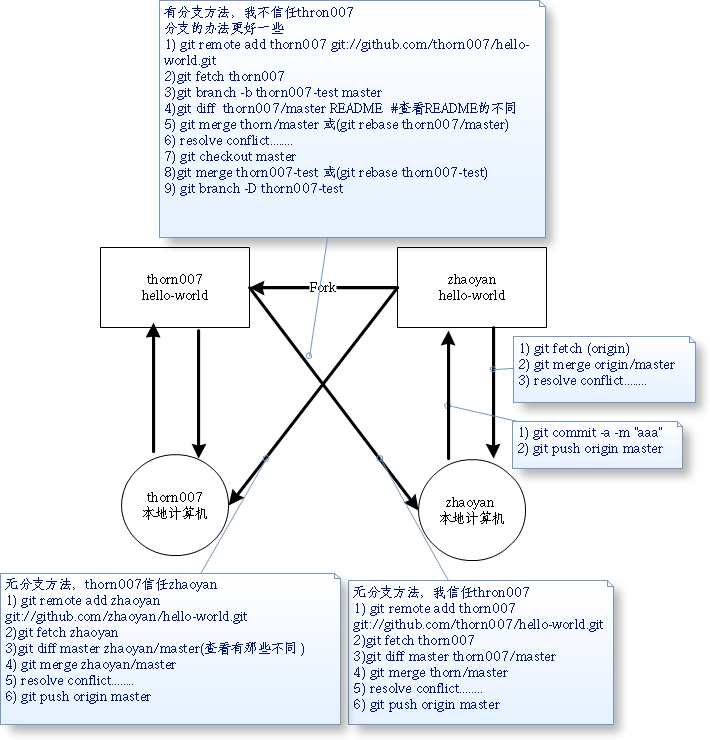
\includegraphics[scale=0.8]{pics/git-corp} \\

% \begin{verbatim}

%
% 下面我给出一个具体的例子:
% 当合作伙伴bob希望改进我(rocrocket)的工作成果,则:
% $git clone /home/rocrocket/project myrepo //此命令用于克隆我的工作到bob的myrepo目录下。请注意,此命令有可能会因为/home/rocrocket的目录权限问题而被拒绝,解决方法是chmod o+rx /home/rocrocket。
% (省略bob数小时的开发过程)…
% $git commit -a //bob提交自己的改进成果到自己的git仓库中,并口头告知我(rocrocket)他已经完成了工作。
%
% 我如果非常信任bob的开发能力:
% $ cd /home/rocrocket/project
% $ git pull /home/bob/myrepo //pull命令的意思是从远端git仓库中取出(git-fetch)修改的代码,然后合并(git-merge)到我(rocrocket)的项目中去。读者要记住一个小技巧,那就是“git pull .”命令,它和git merge的功能是一样的,以后完全可以用git pull .来代替git merge。请注意,git-pull命令有可能会因为/home/bob的目录权限问题而被拒绝,解决方法是chmod o+rx /home/bob。
%
%
% 如果我不是很信任bob的开发能力:
% $ cd /home/rocrocket/project
% $ git fetch /home/bob/myrepo master:bobworks //此命令意思是提取出bob修改的代码内容,然后放到我(rocrocket)工作目录下的bobworks分支中。之所以要放到分支中,而不是 master中,就是要我先仔仔细细看看bob的开发成果,如果我觉得满意,我再merge到master中,如果不满意,我完全可以直接git branch -D掉。
% $git whatchanged -p master..bobworks //用来查看bob都做了什么
% $git checkout master //切换到master分区
% $git merge bobworks
% $git branch -D bobworks //如果我检查了bob的工作后很不满意,就可以用-D来放弃这个分支就可以了
% 过了几天,bob如果想继续帮助我开发,他需要先同步一下我这几天的工作成果,只要在其当初clone的myrepo目录下执行git pull即可:
% #git pull //不用加任何参数,因为当初clone的时候,git已经记住了我(rocrocket)的工作目录,它会直接找到我的目录来取。
% \end{verbatim}
	\begin{itemize}
	\item if modification is small , you can use email+patch; If the modification is big, you can use fork pattern

    \item you can clone a exist project from other's people or on other computers,
	\item Use email topic
		\begin{verbatim}
		1) git clone http://www.bitsun.com/git/gittutorcn.git
		2) edit and commit
		//method 1 (develop on master)
		$ git  fetch origin
		$ git rebase origin
		$ git format path origin  ->0001-your-buddy-s-contribution.txt
		//method 2 (develop on branche, better)
		$ git checkout -b patch_mubs
		$ git checkout master
		$ git pull
		...
		$ git checkout patch_mubs
		$ git rebase master ( why I need rebase here, I want to know answer)
		
		3)email 0001-your-buddy-s-contribution.txt to vortune@gmail.com
		for vortune:
		1) git checkout -b buddy-in
		2) git am /path/to/0001-your-buddy-s-contribution.txt
		
		\end{verbatim}
	\end{itemize}

    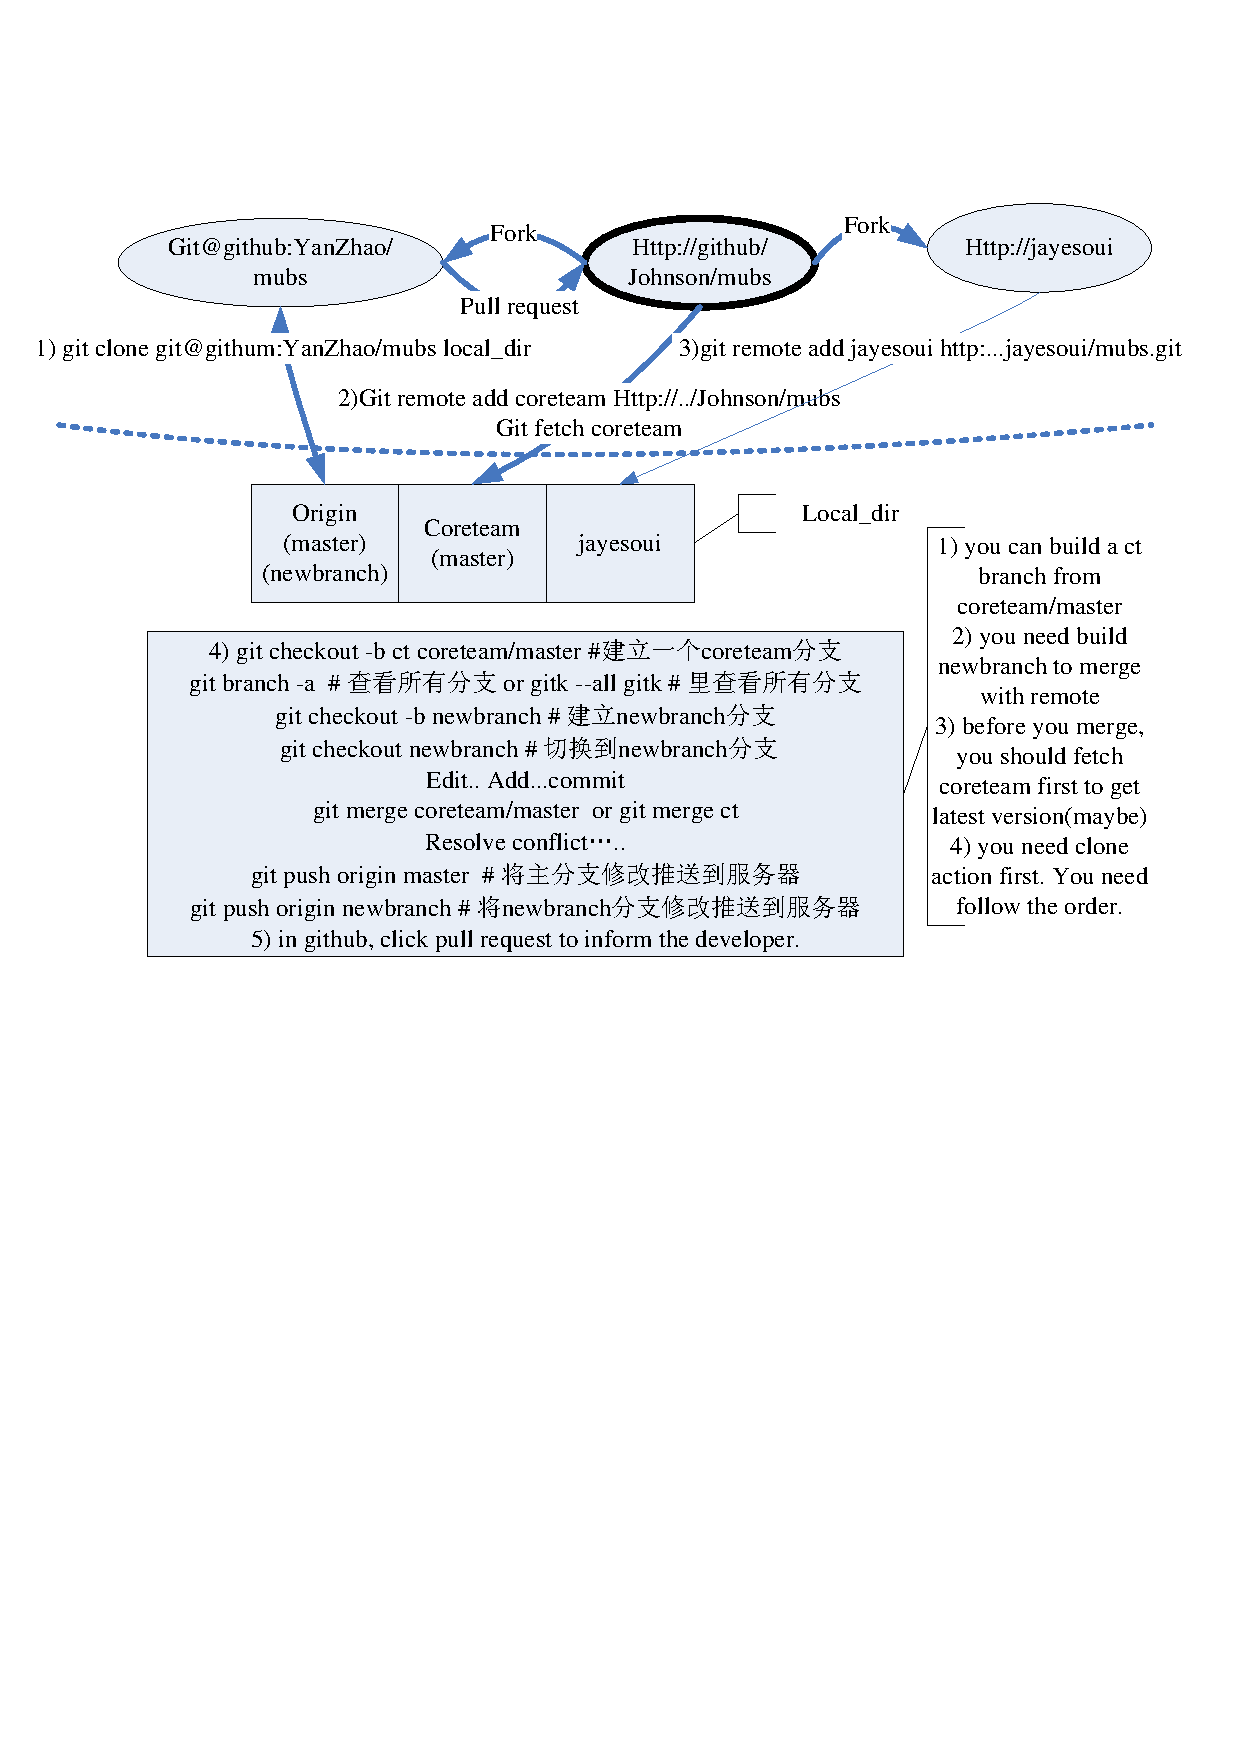
\includegraphics[scale=0.7]{pics/Visio-git_cooperate}



\section{IDE}
If you can access GUI, you can use code::block and kile to develop and documents. if
you login by SSH, By now, I think that best tool is Emacs, with GUD, it can debug a
program. Does Emacs support latex well? Yes, It has tex mode. \par

Windows has VS community version.  Mac has Xcode, but I didn't try it too much. 

In linux, There are many tools you can uses. The most advance tool is Eclipse. the medium tools are codelite and UltraGDB. And the simple tool is vim and gdb( gdb -tui) \\

ddd is old tool, when I use it in mint 17, It's difficult to set font.  It seems that a bug for ddd. and ddd is old tool which seems to stop developing.  \\

Then I try affinic debugger, It's a commercial software and need serial number, I look for and there is not many answers on google, Maybe it's not very popular,  and the shortcoming is white background and you cann't change color theme. so I give it up. \\

codelite is a good tool, Setting->colours and fonts->Customize->C++ , you can select Themes: Monokai\_2, and you can set font MonoSpace 11pt.  
in codelite, you need to set terminal as gnome-terminal in Setting->preferences->terminal "/usr/bin/gnome-terminal -t '\$(TITLE)' -e '\$(CMD)'"
It also use xterm as debugger output. In mint, it output ugly font.  you need to produce .Xresources file on you home directory.  I keep it on the linux software backup. 

UltraGDB is subset of Eclipse, if you just need front-end of GDB, It's the best one. You can set dark theme in Window->Preferences->General->Appearance \\

In conclusion,  front end of GDB are UltraGDB and codelite. IDE are eclipse and codelite.

\subsection{Understand}
Understand is a good tools to read a large scale software. 
\begin{itemize}
\item Don't add .h, .inc, or .inl files into understand project, It will be included by .cpp and analyze automatically. 
\item For C++, use strict option in project configuration. You can adjust c++ version in strict C++ configuration. By now, It's good to use C++11, C++14 is too new
\item In Understand ,you can use "Improve project accuracy"->"missing include files" to help you search head file automatically. 
\item For CMake file, you can use \textbf{CMake -CMAKE\_EXPORT\_COMPILE\_COMMANDS -G "Unix Makefiles"} It will produce a compile\_commands.json file. In the end, you can use \linuxcommand{und} to produce a project.und. It will includes correct configuration information.  Don't use -G "Xcode", It will not produce  compile\_commands.json file.  Detail can be seen in my EverNote bookmark. 
\item For gcc and g++ project, you can use buildspy tool in Understand, detail can be seen in my EverNote bookmark.
\item If you select "terminal" color theme, inactive code will not visiable, you can change the background color to make it visible through "Preferences"->"Editor"->"Styles"
\item When analyze a long or difficult file, "worker process killed after 2 mins", you can try "Ananlyze changed file " again. if 2 minutes is too short, you can configure it longer on this specify file by override configuration. 
\item Macro is key factor in understand project, you can define it maually, but recommended way is to use CMAKE or buildsyp or visual studio to prodce a understand project automatcilly. it will includes all the correct Macro defination and include path. 
\item You can use buildspy to build a understand project in linux, configure project to relative path "Portability" then you can move source code and understand project to Mac, and use understand in Mac to open it. the interface on Mac looks better than Linux. 

\item By now, I have two projects, one is llvm and the other is openuh.  For llvm, when you run CMake in test1 directory, It will produce some head file, when you compile use xcode or makefile, It will produce some def file. But I didn't run can compiling in test1 directory, but I have really compiled src in cmake\_release\_build directory. When i use add automaticlly search headfile, it add some files in cmake\_release\_build directory. In Understand Project Browers, you can see these three directories, in fact, test1 and cmake\_release\_build are overlapped. 

\item for LLVM and openuh, when you configure and compile the source code, It will produced some addtional files to be used in compiling in build directory. so, In the end you understand project will also include build directory in the end. 
  
\end{itemize}





\chapter{Other Tools}






\section{OS and phone}

\subsection{useful tips}
\begin{itemize}
\item In linux or mac, if you want to print c++ source with linenumber, you can use \\
\verb=enscript -MLetter --line-numbers -p - --word-wrap a.cpp | pstopdf -i -o ~/out.pdf=
you can use \verb=brew install enscript= to install enscript. Maybe you will see a error: you can't write /usr/local/etc.
then use \verb=sudo chown -R `whoami`:admin /usr/local/share=to give you permission. and then try brew again. 
\end{itemize}

Common used applications in each OS. in phone, I didn't install many app by now. it make you phone battery die very quickly. and I always sit in front of computer. \\

\begin{tabular}{|c|c|c|c|}
\hline & mac & windows & linux  \\
\hline diagramming & \parbox[c]{10em}{\centering OmniGraff \\ ConceptDraw}& visio & Dia   inkscape \\
\hline vector drawing & illustrator & coreldraw illustrator & ? \\
\hline edit & textmate & Ultraedit & Emacs \\
\hline doc & mactex & Ctex & livetext \\
\hline web & dreamweaver & dreamweaver & ? \\
\hline screenshot & jing snapZ pro & snagit & ? \\
\hline screencast & \parbox[c]{10em}{\centering screen flow \\ camtasia }& camtasia & Xvidcap \\
\hline download & amule or Vuze & emule & amule  \\
\hline audio editor & \parbox[c]{10em}{\centering audacity(amateur) \\ logic(profession)} & \parbox[c]{10em}{\centering gold wave(amateur)\\ adobe audition(professional)} & ? \\
\hline video editor & \parbox[c]{10em}{\centering finalcut \\  imoive(amateur)} & \parbox[c]{10em}{\centering premiere(professional) \\HuiShengHuiYing (amateur)}& ? \\
\hline
\end{tabular}
\subsection{Phone}
\begin{itemize}
  \item In my phone, weibo, webchat and web browser are three information sources.
  \item Evernote is main note tool. It can sync between phone and computer. When you have a lot note in Evernote, you can import them to latex document if you have time.
  \item In phone, you can use Everclip, on computer, you can use Evernote web clipper( in chrome browser)
  \item In Weibo or Webchat, you can repost or share it on moment. That is very easy way to keep knowledge. If this knowledge is just useful for you, you can use Everclip text, download image, or copy URL, Then use share function in your phone to save them to Evernote.
\end{itemize}
\subsection{mac}
\begin{itemize}
 \item command is window key if you use a windows keyboard.
 \item command+~ switches between documents. command+tab switches between applications.
  \item quicksiver can open and close any applications
  \item homebrew can be used to install a lot soft package from git to /usr/local/bin. It's very easy just brew install. 
  if you have older version in /usr/bin, you need to export PATH=/usr/local/bin:\$PATH. It's not very convenient. For this problem, you can down load module software, and use module load and unload, it is  environment management . 
  \begin{verbatim}
  brew install modules 
  \end{verbatim}
  
  \item 
  \begin{tabular}{|p{0.45\textwidth}|p{0.45\textwidth}|}
  \hline command +T & open a new brower \\
  \hline command+T, command + ~ & switch application or windows \\
  \hline command+shift+4 & screen snap \\
  \hline command+option+esc & force app quit(you need to command+tab switch ) \\
  \hline command+h & hide current windows \\
  \hline command+Q or W & close app or windows. \\
  \end{tabular} 
  
\end{itemize}

\subsection{win7}
\begin{itemize}
\item win+arrow key can dock windows to left,right,maximize and minimize, that is very useful
\item win+p can control project camera
\item win+1,2,3 can launch programme in task bar quickly
\item when the explore becomes slowly, you should check tool--manager add-ons to see which add-on is slow.
\item right mouse key can produce a jump list, the content of jump list will change according to the type of progamme.
\item move windows to the left side can change it to 50\% width.
\item win+L to lock the windows
\end{itemize}

\subsection{iexplore and chrome}
\begin{itemize}
\item learn to use tab to explore the internet. that is very useful, don't try to open a new page in a new windows, but in a new tab. \hotkey{ctrl+num} to navigate the tabs. and \hotkey{ctrl+click} to open a link in a new tab. \hotkey{ctrl+T} open a new tab. \hotkey{ctrl+w} to close the current tab.
\end{itemize}






\ifx \allfiles \undefined
%\end{CJK*}


\end{document}
\fi
